\documentclass[12pt, a4paper, onecolumn]{report}

% --- Packages ---
\usepackage[utf8]{inputenc}
\usepackage[T1]{fontenc}
\usepackage{geometry}
\geometry{
    a4paper,
    left=1.2in,
    right=0.8in,
    top=0.8in,
    bottom=0.8in
}
\usepackage{setspace}
\onehalfspacing % 1.5 line spacing (Guideline 3)
\usepackage{titlesec}
\usepackage{graphicx}
\usepackage{amsmath}
\usepackage{amssymb}
\usepackage{listings}
\usepackage{xcolor}
\usepackage{hyperref}
\usepackage{cite}
\usepackage{fancyhdr}
\usepackage{newtxtext,newtxmath} % Times New Roman (Guideline 12)
\usepackage{tikz} % Required for side stripe positioning
\usetikzlibrary{arrows.meta, shapes, positioning, calc}
\usepackage{array}
\usepackage{ragged2e}
\newcolumntype{E}{>{\RaggedRight\ttfamily\small}p{5.2cm}}
\newcolumntype{M}{>{\centering\arraybackslash\small}p{2.2cm}}
\newcolumntype{D}{>{\RaggedRight\arraybackslash\small}X}
\usepackage{caption}
\usepackage{tabularx}
\usepackage{float}
\usepackage{booktabs}

% --- Font Sizes (Guideline 12) ---
\titleformat{\chapter}[display]
  {\normalfont\fontsize{16}{19}\bfseries}{\chaptertitlename\ \thechapter}{10pt}{\Huge}
\titleformat{\section}
  {\normalfont\fontsize{14}{17}\bfseries}{\thesection}{1em}{}
\titleformat{\subsection}
  {\normalfont\fontsize{12}{15}\bfseries}{\thesubsection}{1em}{}
\renewcommand{\normalsize}{\fontsize{12}{15}\selectfont}

% --- Page Numbering (Guideline 4 & 11) ---
\fancyhf{}
\fancyfoot[C]{\thepage}
\pagestyle{plain}

% --- Code Styling ---
\definecolor{codegreen}{rgb}{0,0.6,0}
\definecolor{codegray}{rgb}{0.5,0.5,0.5}
\definecolor{codepurple}{rgb}{0.58,0,0.82}
\definecolor{backcolour}{rgb}{0.95,0.95,0.92}

\lstset{
    backgroundcolor=\color{backcolour},  
    commentstyle=\color{codegreen},
    keywordstyle=\color{magenta},
    numberstyle=\tiny\color{codegray},
    stringstyle=\color{codepurple},
    basicstyle=\ttfamily\footnotesize,
    breakatwhitespace=false,        
    breaklines=true,                
    captionpos=b,                    
    keepspaces=true,                
    numbers=left,                    
    numbersep=5pt,                  
    showspaces=false,                
    showstringspaces=false,
    showtabs=false,                  
    tabsize=2
}

\begin{document}
\pagenumbering{roman}

% --- 1. Title Page ---
\begin{titlepage}
    \centering
    \textbf{eMETER -- ELECTRICITY BILLING AND METER MANAGEMENT SYSTEM}
   
    \vspace{1.5cm}
    \fontsize{14}{17}\selectfont
    \textbf{DISSERTATION}\\
    SUBMITTED IN PARTIAL FULFILLMENT OF THE REQUIREMENTS\\
    FOR THE AWARD OF THE DEGREE OF\\
   
    \vspace{1.5cm}
    \fontsize{16}{19}\selectfont
    \textbf{Master of Computer Applications}\\[0.5em]
    \textbf{MCA}
   
    \vspace{1.5cm}
    \fontsize{12}{15}\selectfont
    By\\
    \textbf{Anas Julfikar}
   
    \vspace{1cm}
    % \includegraphics[width=0.3\textwidth]{LOGO.jpeg}
   
    \vspace{1cm}
    \fontsize{12}{15}\selectfont
    \textbf{DEPARTMENT OF COMPUTER SCIENCE}\\
    \textbf{ALIGARH MUSLIM UNIVERSITY}\\
    \textbf{ALIGARH (INDIA)}
   
    \vfill
    \fontsize{12}{15}\selectfont
    \textbf{Year of submission: 2026}

    % --- Side Stripe ---
    \begin{tikzpicture}[remember picture, overlay]
        \node[rotate=90, anchor=west] at ([xshift=1cm, yshift=-4cm]current page.west) {\fontsize{10}{12}\selectfont Anas Julfikar};
        \node[rotate=90, anchor=west] at ([xshift=1cm, yshift=-12cm]current page.west) {\fontsize{10}{12}\selectfont eMeter System};
        \node[rotate=90, anchor=west] at ([xshift=1cm, yshift=-22cm]current page.west) {\fontsize{10}{12}\selectfont 2026};
    \end{tikzpicture}
\end{titlepage}

% --- 2. Certificate ---
\newpage
\begin{center}
    \Huge \textbf{CERTIFICATE}
\end{center}
\vspace{1cm}
This is to certify that the dissertation/project work entitled \textbf{``eMeter -- Electricity Billing and Meter Management System''} being submitted by \textbf{Mr. Anas Julfikar} in partial fulfillment of the requirements for the award of the \textbf{Master of Computer Applications (MCA)} degree of Aligarh Muslim University, Aligarh, is a record of the student's own work, carried out under my supervision and guidance.

It is further certified that the student has worked on the \textbf{eMeter} system, at \textbf{Aligarh Muslim University} for completion of this work from \textbf{January 2026} to \textbf{July 2026}.

\vspace{3cm}
\noindent
Signature \\
(of the supervisor) \\


% --- 3. Acknowledgement ---
\newpage
\chapter*{ACKNOWLEDGMENT}
\addcontentsline{toc}{chapter}{Acknowledgment}
The completion of this dissertation marks the end of a long and deeply personal journey; one that began with an idea and was carried forward through months of dedication, late nights, and the quiet determination that grows in the presence of people who truly care.
\vspace{1em}
First and foremost, I express my profound gratitude to Almighty Allah, the Most Gracious and Most Merciful, for blessing me with the health, strength, and patience to complete this journey. Every step forward has been by His grace.
\vspace{1em}
I extend my sincere thanks to my supervisor, Prof. Aasim Zafar, Department of Computer Science, Aligarh Muslim University, for his guidance, support, and thoughtful mentorship. His expertise brought academic clarity to this work, and his encouragement provided direction whenever the path felt uncertain.
\vspace{1em}
I am also grateful to the Department of Computer Science, Aligarh Muslim University, and its faculty and staff for providing the academic environment and resources necessary to complete this Master of Computer Applications programme.
\vspace{1em}
I would like to express my special thanks to Dr. Faraz Masood for his invaluable contribution, guidance, and help. His support as both a faculty member and an older brother has been instrumental in the successful completion of this work.
\vspace{1em}
Building \textbf{eMeter} extended beyond a formal academic task, offering an opportunity to apply theoretical knowledge in a practical context. It demanded consistent effort, careful design decisions, and a grounded approach to addressing real-world challenges within the utility management domain.

% --- 4. Contents ---
\newpage
\tableofcontents
\listoffigures
\listoftables

% --- 5. Abstract ---
\newpage
\chapter*{ABSTRACT}
\addcontentsline{toc}{chapter}{Abstract}

Efficient electricity billing and utility management are essential for modern infrastructure systems. However, traditional electricity billing methods still rely heavily on manual meter reading, paper-based records, delayed bill generation, and fragmented administrative workflows. These limitations often result in operational inefficiencies, human errors, revenue leakage, and reduced consumer transparency, especially in areas with poor network connectivity.

This dissertation presents \textbf{eMeter}, a comprehensive Electricity Billing and Meter Management System designed to automate and modernize the complete utility billing workflow. The system follows a three-tier architecture consisting of a \textbf{Django REST Framework} backend, a \textbf{React 18} web dashboard for administrative management, and an offline-first \textbf{React Native} mobile application for field meter readers. \textbf{PostgreSQL} is used for secure and scalable data storage.

A major contribution of the proposed system is its resilient offline synchronization mechanism. Using \textbf{AsyncStorage} and the \textbf{NetInfo} API, the mobile application enables meter readers to capture readings without internet connectivity and automatically synchronize the data once connectivity is restored. This ensures uninterrupted field operations and reliable data consistency.

The system also implements a dynamic \textbf{BillingSettings} policy engine that automates electricity bill calculation, including energy charges, fixed charges per kilowatt of load, electricity duty, meter rent, arrears, and late payment surcharges. Additional features include a \textbf{Consumer Self-Service Portal} for end-user access to billing history and PDF invoices, bulk meter reading import via Excel spreadsheets with automatic bill generation, server-side \textbf{PDF bill generation}, role-based authentication, analytics dashboards, and integrated \textbf{WhatsApp bill sharing}.

By digitizing the complete billing lifecycle, eMeter significantly improves operational efficiency, reduces human error, and enhances transparency in utility management. The scalable architecture of the system also provides a strong foundation for future integration with \textbf{Smart Meter} and \textbf{IoT-based} utility systems.

\clearpage
\pagenumbering{arabic}

% --- 6. Chapters ---

\chapter{INTRODUCTION}

\section{Background}
Utility billing and meter management form the financial backbone of electricity providers worldwide. Accurately capturing electricity consumption, calculating usage tariffs, and delivering timely bills are essential operations. Traditionally, these processes have been labor-intensive, relying heavily on paper-based ledger systems or fragmented legacy software. Field workers physically visit consumer premises, record readings manually, and later transfer the data to central servers. This disjointed workflow introduces significant delays, human errors, and vulnerabilities to tampering.

Modernizing this infrastructure requires a cohesive, cross-platform software solution capable of handling distributed field data collection alongside centralized administrative control. eMeter is conceived as a comprehensive end-to-end platform bridging the gap between on-field meter readers, centralized billing administrators, and end consumers. By leveraging modern web and mobile frameworks, the project introduces a highly efficient, automated billing calculation engine driven by dynamic tariff policies.

\section{Literature Survey}
\subsection{Previous Related Work}
Historically, electricity billing systems transitioned from fully manual bookkeeping to computerized batch processing systems in the late 1990s. Early digital utility management systems primarily consisted of isolated desktop applications. With the advent of cloud computing, utility providers began migrating to centralized web portals. However, these systems largely ignored the field operations---meter reading remained a disconnected process using expensive proprietary handheld devices.

More recently, the ubiquity of smartphones has encouraged the adoption of mobile utility apps. Yet, many existing solutions assume a constant internet connection, which is not viable in rural or network-congested areas. Research in mobile distributed systems has increasingly emphasized the need for offline-first architectures in enterprise applications. Techniques involving local caching (e.g., SQLite, AsyncStorage) combined with background synchronization have proven effective in maintaining data integrity across intermittent networks.

\subsection{Project Context}
The eMeter project is developed within the context of a modern, decoupled software architecture. The backend is built using Python and the Django REST Framework, ensuring high security and rapid API development. The administrative dashboard utilizes React 18 and Vite for a highly responsive single-page application (SPA) experience. The mobile client is built using React Native and Expo, which allows cross-platform deployment to both Android and iOS while enabling direct access to native device features and local storage (for offline queueing). A dedicated consumer-facing self-service portal, also built with React 18, enables end users to independently access their billing records.

\section{Present State of Art and its Shortcoming}
The current state of utility billing applications exhibits several significant shortcomings that impede operational efficiency and financial accuracy:
\begin{itemize}
    \item \textbf{High Connectivity Dependency}: Most modern mobile billing applications are built on a traditional synchronous request-response model. These apps frequently fail when the cellular network drops or becomes unstable in remote areas. Without a robust local persistence layer, field workers are often unable to submit readings, leading to data loss, forced repeat visits to the consumer premises, and significant delays in the billing cycle.
    \item \textbf{Rigid and Static Billing Logic}: Legacy billing systems often incorporate tariff structures, tax brackets, and fixed charges as hardcoded constants within the application source code. This architectural rigidity means that whenever government policies or utility rates change, a complete software redeployment is required. This ``update friction'' leads to periods where bills are calculated using obsolete rates, resulting in financial discrepancies and consumer disputes.
    \item \textbf{Fragmented and Siloed Ecosystems}: Utility providers frequently rely on a patchwork of disconnected software solutions---one for consumer registration, another for meter reading, and a third for financial reporting. This fragmentation creates ``data silos'' where information must be manually reconciled or moved via complex ETL (Extract, Transform, Load) processes. The lack of a ``Single Source of Truth'' results in data inconsistency and prevents administrators from gaining real-time visibility into revenue and usage trends.
    \item \textbf{Inefficient Physical Delivery Models}: The reliance on physical bill printing and manual delivery is both costly and environmentally unsustainable. The ``Revenue Realization Gap''---the time between consumption and payment---is unnecessarily widened by the logistical delays of postal or manual delivery. Furthermore, many existing systems lack integrated digital delivery channels like WhatsApp or SMS, which are preferred by modern consumers for immediate record-keeping.
    \item \textbf{No Consumer Self-Service}: Traditional utility systems provide consumers with no direct access to their billing data. Consumers must contact the billing office in person or by phone to query a bill or obtain a copy of an invoice, creating unnecessary administrative overhead for both parties.
\end{itemize}

\section{Introduction of Problem or Work to be Taken up}
This dissertation addresses the systemic and technical inefficiencies in current electricity billing pipelines by developing a unified, cross-platform ecosystem. The work undertaken involves the engineering of a scalable ``Monorepo'' architecture that bridges on-field data collection with centralized administrative control. The core problems and technical objectives addressed in this project include:
\begin{enumerate}
    \item \textbf{Engineering an Offline-First Mobile Client}: Developing a React Native application that ensures zero data loss by securely queueing meter readings in local storage (AsyncStorage). The challenge involves implementing a non-blocking synchronization algorithm that detects network availability (via NetInfo) and manages eventual consistency with the server.
    \item \textbf{Dynamic Tariff and Policy Management}: Implementing a backend \texttt{BillingSettings} engine that allows for the runtime configuration of per-unit rates, fixed connection charges, electricity duty percentages, and meter rent. This eliminates the need for source code modification during policy shifts.
    \item \textbf{Automated Multi-Channel Bill Generation}: Creating a high-performance Python-based service for the real-time calculation of consumption charges, generation of print-ready PDF invoices using \textit{xhtml2pdf}, and automated delivery via the WhatsApp API.
    \item \textbf{Identity and Access Management}: Implementing a granular Role-Based Access Control (RBAC) system using JWT (JSON Web Tokens) to ensure that Administrators, Meter Readers, and Consumers have restricted and secure access to their respective modules.
    \item \textbf{Bulk Data Import via Excel}: Providing administrators with an Excel-based import workflow for batch submission of meter readings, enabling mass bill generation from structured spreadsheet data without manual entry.
    \item \textbf{Consumer Self-Service Portal}: Developing a dedicated web interface for end consumers to independently view their meter reading history, access generated bills, and download PDF invoices, thereby reducing administrative overhead and improving transparency.
\end{enumerate}

\section{Broad Outline of the Work}
This dissertation is structured to provide a comprehensive walkthrough of the eMeter ecosystem, from initial motivation to technical implementation and future potential. The chapters are organized as follows:
\begin{itemize}
    \item \textbf{Chapter 1 (Introduction)}: Sets the stage by outlining the historical context of utility management, conducting a thorough literature survey of current technologies, and defining the specific shortcomings that eMeter aims to resolve.
    \item \textbf{Chapter 2 (Problem Formulation)}: Deep-dives into the technical aspects of the problem, focusing on the significance of the ``Offline-First'' paradigm, the mathematical complexities of billing, and the proposed method of solution through a decoupled full-stack architecture.
    \item \textbf{Chapter 3 (System Analysis and Design)}: Details the architectural blueprint, including the three-tier model, the normalized PostgreSQL database schema, the API workflow diagrams, and the functional/non-functional requirements of each system actor.
    \item \textbf{Chapter 4 (System Implementation and Testing)}: Covers the actual development process, highlighting the use of Django REST Framework for secure APIs, React for the admin and consumer dashboards, and React Native for the mobile sync logic. It also presents the results of unit, integration, and performance testing.
    \item \textbf{Chapter 5 (Application and Scope)}: Explores the real-world deployment scenarios for eMeter, its adaptability to other utility types (water/gas), and a detailed roadmap for integrating IoT-based Smart Meters.
    \item \textbf{Chapter 6 (Conclusion)}: Summarizes the project's achievements, acknowledges its current limitations, and outlines future research directions to further modernize utility infrastructure.
\end{itemize}


\chapter{PROBLEM FORMULATION}

\section{Various Aspects of the Problem}
The eMeter system attempts to resolve several multifaceted engineering and business logic challenges inherent to utility management.

\subsection{The Network Unreliability and Data Persistence Challenge}
Meter readers operate in diverse and often hostile network environments, including basements, rural sectors, and high-density residential complexes where cellular reception is highly unstable or non-existent. A traditional ``Cloud-Only'' mobile application that relies on immediate API responses will experience high failure rates in these conditions. The engineering challenge lies in formulating a ``Local-First'' architecture that treats the mobile device as a temporary source of truth, utilizing persistent local storage to queue readings and implementing a robust background synchronization engine that guarantees eventual consistency without data duplication or loss.

\subsection{Complex Billing Mathematics and Policy Modeling}
Electricity billing involves a sophisticated set of variables that change based on government regulations and consumer categories. This includes fixed connection charges based on sanctioned load (kilowatts), variable per-unit energy rates, electricity duty percentages, meter rental fees that vary by phase (single or three-phase), and potential late payment surcharges. Modeling these variables as a dynamic policy engine rather than hardcoded logic is a significant mathematical and database design problem. The system must compute these values in real-time while allowing administrators to modify the underlying tariff policies via a web interface.

\subsection{Cross-Platform Rendering and Output Fidelity}
A major functional requirement is the generation of professional, print-ready PDF bills. However, ensuring that the visual representation of a bill remains consistent across the web dashboard (HTML/CSS), the mobile preview (React Native components), and the final generated PDF (\textit{xhtml2pdf}) is a significant rendering challenge. This requires a unified billing data model and a server-side templating engine capable of producing high-fidelity documents that meet formal utility standards.

\subsection{Consumer Data Access and Self-Service}
A persistent problem in traditional billing systems is the absence of a consumer-facing interface. Consumers cannot independently verify their consumption data or obtain a copy of their bills without direct contact with the billing department. The challenge involves building a secure, role-isolated portal that allows consumers to access only their own data while preventing unauthorized cross-consumer data access.

\subsection{Security and Granular Access Control}
Managing a distributed system with multiple actors (Administrators, Field Workers, and Consumers) introduces complex security requirements. The system must implement a strict Role-Based Access Control (RBAC) layer to ensure that sensitive consumer data is protected. For instance, a Meter Reader should only have access to consumer lookup and reading submission, while an Administrator requires full control over billing policies and financial reports. Implementing this across web and mobile clients using secure token-based authentication (JWT) is a core aspect of the problem.

\section{Significance of the Work}
The implementation of the eMeter system holds significant value as a catalyst for the digital transformation of traditional utility management infrastructure. By replacing fragmented, paper-based, or legacy manual workflows with a unified, high-performance ecosystem, the project addresses critical gaps in revenue protection, operational agility, and consumer trust. The significance of this work extends beyond mere process automation; it provides a data-driven framework that empowers utility providers with real-time operational insights while ensuring that consumers are served with unprecedented transparency and modern digital convenience.

\subsection{Operational Efficiency}
By digitizing the entire flow from meter reading to bill delivery, utility companies can reduce the billing cycle from weeks to minutes. Field workers can record meters without worrying about network connectivity, and administrators can monitor collections in real-time through the analytics dashboard. The Excel bulk import feature further accelerates operations by enabling mass bill generation from existing spreadsheet data.

\subsection{Transparency and Consumer Empowerment}
The Consumer Self-Service Portal grants end users direct, on-demand access to their billing records and reading history. Consumers can independently download PDF invoices at any time, eliminating the need to contact the billing office for routine enquiries. This transparency builds trust and significantly reduces dispute volume.

\section{Proposed System and Method of Solution}
The proposed solution is the \textbf{eMeter Full-Stack Platform}, a unified, cross-platform ecosystem designed to address the end-to-end requirements of modern utility management. The platform is engineered using a decoupled, service-oriented architecture that ensures high scalability, resilient field operations, and centralized administrative control.

\subsection{Architectural Paradigm: Decoupled Service-Oriented Design}
To achieve maximum flexibility and performance, the system is partitioned into three distinct yet highly integrated layers:
\begin{itemize}
    \item \textbf{Data Tier (PostgreSQL)}: A robust relational database that serves as the ``Single Source of Truth,'' enforcing data integrity through normalized schemas and referential constraints.
    \item \textbf{Business Logic Tier (Django REST Framework)}: A secure, Python-powered API gateway that handles authentication, billing mathematics, document rendering, and complex transaction management.
    \item \textbf{Presentation Tier (React \& React Native)}: A multi-client strategy involving a responsive admin web dashboard, a dedicated consumer self-service portal, and an optimized mobile client for on-field operations.
\end{itemize}

\subsection{The Offline-First Field Operations Methodology}
To solve the critical challenge of network unreliability in field operations, eMeter adopts an ``Offline-First'' synchronization methodology. The React Native mobile client utilizes a local persistence layer built with \textbf{AsyncStorage} to cache consumer data and capture readings locally.
\begin{enumerate}
    \item \textbf{Local Queue Management}: Every meter reading is initially stored as a serialized JSON object in the device's local memory, guaranteeing zero data loss regardless of network state.
    \item \textbf{Network State Awareness}: The system integrates the \textbf{NetInfo API} to continuously monitor the device's connectivity status.
    \item \textbf{Asynchronous Synchronization Queue}: Upon detecting an active internet connection, a non-blocking background service initiates a ``Sync'' sequence. This service serially transmits pending records to the backend, handles potential data collisions, and updates the local state once server acknowledgment is received.
\end{enumerate}

\subsection{Dynamic Billing Logic and Policy-Driven Calculation}
The core financial engine of eMeter is designed around a dynamic policy-driven calculation engine. Unlike traditional systems that hardcode billing rates, eMeter utilizes a \texttt{BillingSettings} model on the backend.
\begin{itemize}
    \item \textbf{Policy Configuration}: Administrators can define the per-unit energy rate, fixed connection fee per kilowatt of sanctioned load, electricity duty percentage, single-phase meter rent, and three-phase meter rent via the web interface.
    \item \textbf{Automated Calculation Service}: When a reading is submitted or synchronized, a specialized Python service is triggered. It performs a ``snapshot'' look-up of the current active policy, computes the consumption differential, applies the relevant charges, and generates a finalized \textbf{Bill} record. This ensures that every bill is calculated accurately based on the policy active at that specific timestamp (Policy Snapshotting).
\end{itemize}

\subsection{Excel-Based Bulk Import and Automated Bill Generation}
A critical administrative workflow in eMeter is the bulk reading import feature. Administrators can upload an Excel spreadsheet (\texttt{.xlsx} or \texttt{.xls}) containing multiple consumer readings. The system automatically detects the column layout (3-column or 4-column format), validates each row, and generates a bill for every successfully processed reading. A detailed result panel reports successes and per-row error messages, enabling rapid error correction.

\subsection{Consumer Self-Service Portal}
The Consumer Portal is a distinct, independently authenticated React 18 web application. Consumers log in using their consumer number and a personal password. Once authenticated, they can view their complete meter reading history, check the status of all bills (paid, unpaid, overdue), and download any bill as a professionally formatted PDF invoice. The portal is entirely read-only for consumers, enforcing strict data isolation so that each user can access only their own records.

\subsection{Asynchronous Document Orchestration and Multi-Channel Delivery}
The final stage of the solution involves the automated generation and distribution of billing documents. The system leverages \textbf{xhtml2pdf} for server-side HTML-to-PDF rendering, injecting live billing data into a standardized invoice template. For administrative reporting, \textbf{openpyxl} is used to generate comprehensive Excel workbooks. The platform completes the lifecycle by integrating the \textbf{WhatsApp API}, allowing field workers or administrators to share generated PDF bills directly with consumers.

\subsection{Integrated Security and Role-Based Identity Management}
The solution is secured by a robust Identity Management layer. Utilizing \textbf{JSON Web Tokens (JWT)}, the system enforces strict Role-Based Access Control (RBAC). This ensures that each actor (Administrator, Meter Reader, Consumer) is presented with a tailored interface and has access only to the data and operations necessary for their role, protecting the privacy and integrity of the overall system.

\chapter{SYSTEM ANALYSIS}

\section{Introduction}

System Analysis and Design is one of the most critical phases in the development of the proposed Electricity Meter Reading and Billing System (eMeter). This phase focuses on understanding the operational requirements of electricity billing organizations, identifying the limitations of traditional billing approaches, and designing a modern automated solution capable of handling consumer management, meter reading collection, bill generation, payment tracking, and analytical reporting in an efficient manner.

The proposed system has been designed as a centralized digital platform that integrates a web-based administrative dashboard, a consumer self-service portal, and a mobile application for field workers. The architecture emphasizes scalability, security, reliability, and ease of use while ensuring that electricity billing operations can be conducted efficiently even in areas with unstable internet connectivity.

The design methodology adopted for this project follows a modular and service-oriented approach where each component performs a specialized task while maintaining seamless communication with the remaining modules through RESTful APIs. The system utilizes PostgreSQL as the relational database management system, Django REST Framework as the backend API layer, React 18 for the administrative web dashboard and consumer portal, and React Native for the mobile meter reading application.

\section{Information Gathering}

The development of the proposed Electricity Meter Reading and Billing System (eMeter) was preceded by a comprehensive process of information gathering intended to understand the operational workflow, administrative challenges, field-level difficulties, and billing requirements associated with electricity distribution and utility management systems.

The objective of this phase was not limited to collecting general background information regarding electricity billing procedures. Instead, the primary focus was to study real-world operational scenarios involved in electricity meter reading, bill generation, revenue collection, consumer management, and administrative monitoring so that these practical requirements could be translated into an efficient digital system architecture.

The information gathering process focused on several critical areas including the organizational structure of electricity billing operations, user roles and responsibilities, billing workflows, field-level meter reading challenges, reporting requirements, and technical infrastructure limitations.

\subsection{Study of Organizational Structure}
Electricity distribution organizations generally operate through a hierarchical administrative structure where responsibilities are distributed among multiple operational levels. The organizational workflow observed during the analysis phase follows a structured administrative hierarchy as illustrated in Figure 3.1.

\begin{figure}[htbp]
    \centering
    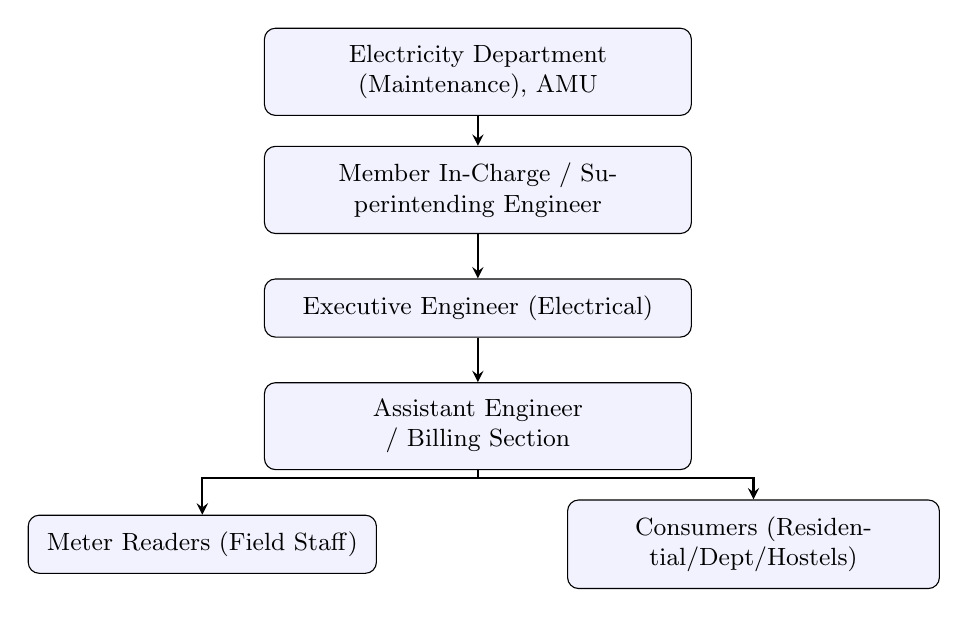
\begin{tikzpicture}[
        node distance=1.5cm,
        every node/.style={rectangle, draw, rounded corners, fill=blue!5, inner sep=6pt, text width=5cm, align=center, font=\small},
        arrow/.style={thick, ->, >=stealth}
    ]
        \node (root) {Electricity Department (Maintenance), AMU};
        \node (admin) [below of=root] {Member In-Charge / Superintending Engineer};
        \node (exec) [below of=admin] {Executive Engineer (Electrical)};
        \node (billing) [below of=exec] {Assistant Engineer / Billing Section};
        \node (field) [below of=billing, xshift=-3.5cm, text width=4cm] {Meter Readers (Field Staff)};
        \node (consumer) [below of=billing, xshift=3.5cm, text width=4.3cm] {Consumers (Residential/Dept/Hostels)};

        \draw [arrow] (root) -- (admin);
        \draw [arrow] (admin) -- (exec);
        \draw [arrow] (exec) -- (billing);
        \draw [arrow] (billing.south) -- ++(0,-0.1) -| (field.north);
        \draw [arrow] (billing.south) -- ++(0,-0.1) -| (consumer.north);
    \end{tikzpicture}
    \caption{Organizational Structure of Electricity Distribution}
\end{figure}

Each level within this hierarchy performs distinct operational functions and requires access to different categories of data. Administrative officers require complete visibility into billing records, payment reports, consumer databases, and operational analytics, whereas field meter readers only require access to assigned consumers and reading submission interfaces. Consumers require a read-only view of their own billing data.

The study revealed that role-based access control is a critical requirement for the proposed system. Different users may perform similar operations while still requiring different levels of data accessibility depending on their administrative responsibilities and operational boundaries.

\subsection{Study of Existing Billing Workflow}

A detailed analysis of traditional electricity billing workflows was conducted to identify operational inefficiencies and manual bottlenecks. The study revealed that in many conventional systems, meter readers manually visit consumer locations, record readings either on paper or handheld devices, and later transfer the collected information into centralized billing software.

This process introduces multiple operational problems including delayed bill generation, data redundancy, inaccurate reading entry, calculation errors, and increased administrative workload. Since billing calculations are often dependent on manual verification processes, the overall billing cycle becomes significantly slower and more error-prone.

The information collection phase also identified that communication between field workers and administrative offices is often fragmented. Administrators frequently lack real-time visibility into completed readings, pending consumer visits, and billing progress, thereby reducing operational transparency.

\subsection{Analysis of Field-Level Operational Challenges}
A critical component of the information-gathering phase involved the identification of infrastructural constraints faced by field workers. The study revealed that meter readers frequently operate in ``shadow zones''---areas with intermittent or non-existent cellular connectivity, such as building basements or high-density residential sectors. In such environments, traditional synchronous data transmission models fail, leading to significant operational bottlenecks and data volatility.

The necessity for an \textbf{Offline-First Architecture} was identified as the primary mitigation strategy. By decoupling the data entry process from the network state, the system ensures that meter reading collection can proceed uninterrupted, with data being persisted locally on the mobile device. Figure 3.2 illustrates the logical workflow of the implemented synchronization mechanism.

\begin{figure}[htbp]
    \centering
    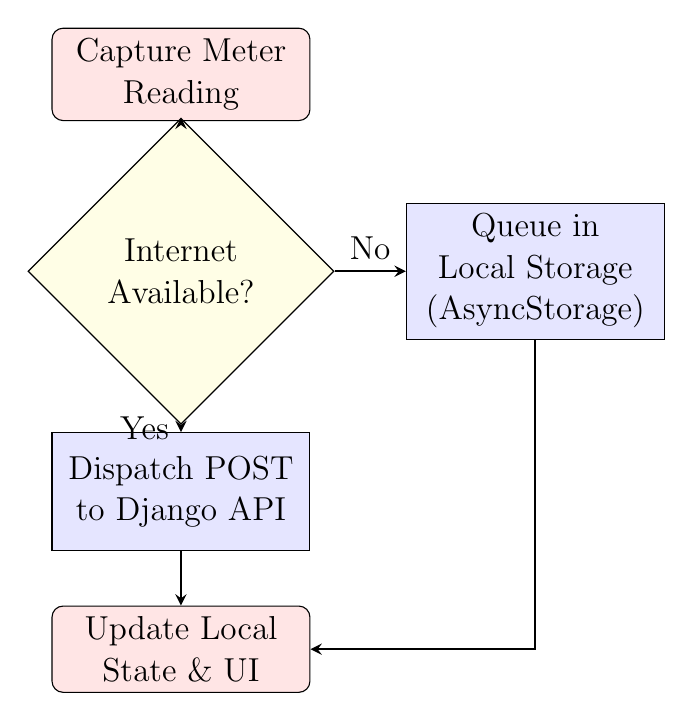
\begin{tikzpicture}[
        node distance=2cm,
        startstop/.style={rectangle, rounded corners, draw, fill=red!10, text width=3cm, align=center, minimum height=1cm},
        process/.style={rectangle, draw, fill=blue!10, text width=3cm, align=center, minimum height=1.5cm},
        decision/.style={diamond, draw, fill=yellow!10, text width=3cm, align=center, inner sep=0.5pt},
        arrow/.style={thick, ->, >=stealth}
    ]
        \node (start) [startstop] {Capture Meter Reading};
        \node (net) [decision, below of=start, yshift=-0.5cm] {Internet Available?};
        \node (local) [process, right of=net, xshift=2.5cm] {Queue in Local Storage (AsyncStorage)};
        \node (api) [process, below of=net, yshift=-0.8cm] {Dispatch POST to Django API};
        \node (success) [startstop, below of=api] {Update Local State \& UI};

        \draw [arrow] (start) -- (net);
        \draw [arrow] (net) -- node[anchor=south] {No} (local);
        \draw [arrow] (net) -- node[left] {Yes} (api);
        \draw [arrow] (api) -- (success);
        \draw [arrow] (local.south) |- (success.east);
    \end{tikzpicture}
    \caption{Offline-First Synchronization Workflow}
\end{figure}

The analysis further derived several high-priority operational requirements:
\begin{itemize}
    \item \textbf{Latent-Search Capabilities}: Implementation of high-performance, local indexing to enable instantaneous consumer lookup even when the device is disconnected from the central server.
    \item \textbf{Minimal Interaction Design}: Adoption of a streamlined UI/UX paradigm that reduces the number of taps required to complete a reading, utilizing autofocus on input fields and smart defaults to minimize cognitive fatigue during high-volume field operations.
    \item \textbf{Schema Validation}: Development of strict client-side validation logic that enforces consumption boundaries, ensuring that current readings are logically subsequent to historical data and preventing the submission of lower values that could disrupt financial calculations.
    \item \textbf{Data Consistency}: Enforcement of atomic synchronization protocols to ensure that submissions are treated as a single unit of work, utilizing idempotent API design to eliminate the risk of duplicate record creation during intermittent network conditions.
    \item \textbf{Offline Export}: The ability to export the unsynced reading queue as an Excel file so that administrators can manually import the data via the web dashboard if synchronization fails persistently.
\end{itemize}

This structured analysis directly informed the development of the React Native mobile client and the background synchronization module, ensuring the system remains robust under real-world infrastructure constraints.


\subsection{Study of Billing and Revenue Requirements}

The information collection process further focused on understanding the financial and billing requirements of electricity distribution organizations. Different electricity providers implement varying tariff structures involving fixed charges, per-unit energy charges, duty percentages, meter rent, and late payment penalties.

The study revealed that billing configurations frequently change according to government regulations and organizational policies. Therefore, hardcoded billing formulas would significantly reduce system maintainability and flexibility.

To address this issue, the proposed system implements a dynamic \textbf{BillingSettings} policy engine that allows administrators to configure tariff structures and billing rules directly from the administrative dashboard without modifying the application source code.

\subsection{Study of Reporting and Administrative Requirements}

Administrative reporting was identified as another critical requirement during the information gathering process. Utility organizations require regular access to analytical reports related to:
\begin{itemize}
    \item Total revenue collection
    \item Pending dues
    \item Consumer statistics
    \item Reading completion status
    \item Monthly billing summaries
    \item Payment histories
\end{itemize}

The study highlighted the importance of centralized dashboards and exportable reports for improving decision-making and operational monitoring. As a result, the proposed system integrates graphical analytics dashboards and Excel export functionality using the OpenPyXL library.

\subsection{Technology Requirement Analysis}
The final phase of information gathering focused on identifying an optimal technology stack capable of supporting the project's requirements for scalability, high availability, data integrity, and a premium user experience. After a rigorous evaluation of modern frameworks, the following technologies were selected to form the eMeter ecosystem:

\begin{itemize}
    \item \textbf{Django REST Framework (DRF)}: Selected as the primary backend engine for its robust ORM, rapid API development cycle, and superior handling of complex business logic.
    \item \textbf{PostgreSQL 16}: Utilized for its ACID compliance, advanced indexing, and reliable relational data management, ensuring the absolute integrity of consumer and billing records.
    \item \textbf{React 18}: Employed for both the administrative dashboard and the consumer self-service portal to provide a highly responsive, state-managed Single Page Application (SPA) experience using modern hooks and concurrent rendering.
    \item \textbf{React Native with Expo}: Chosen for the mobile field module to enable cross-platform deployment while maintaining direct access to native device features and local hardware-level storage.
    \item \textbf{Advanced Security Model (JWT + CSRF)}: To ensure a high security posture, the system implements a multi-layered authentication and authorization framework. While \textbf{JSON Web Tokens (JWT)} handle stateless authorization across distributed clients, the system is further hardened with \textbf{CSRF (Cross-Site Request Forgery)} protection and secure, \textbf{HttpOnly} cookie-based token persistence. This hybrid approach mitigates common vulnerabilities like XSS (Cross-Site Scripting) and unauthorized session hijacking, ensuring that both web and mobile transactions remain protected under a zero-trust model.
\end{itemize}
The information gathering phase played a foundational role in shaping the overall architecture and implementation strategy of the proposed system. The observations and operational insights collected during this phase directly influenced system design decisions, database modeling, security mechanisms, synchronization workflows, and module organization throughout the development lifecycle.

\section{Existing System Analysis}

In many electricity distribution organizations, billing operations are still partially dependent on manual workflows and fragmented software systems. Meter readers physically visit consumer locations, record readings on paper or handheld devices, and later transfer the information into centralized billing software. Such approaches introduce multiple operational inefficiencies and significantly increase the possibility of human error.

Traditional billing systems suffer from delayed bill generation because readings must first be collected manually and then entered into the system at a later stage. This delay often results in billing backlogs, inaccurate consumption calculations, and poor service delivery. Additionally, paper-based systems are highly vulnerable to data loss, duplication, and unauthorized modification.

Another major issue observed in conventional systems is the absence of real-time synchronization between field operations and administrative departments. Administrators frequently lack visibility into completed readings, pending consumer visits, and outstanding payment information. This creates operational bottlenecks and limits decision-making capabilities.

Most existing systems also lack proper authentication and role-based access control mechanisms. Insecure handling of billing records may expose sensitive consumer information and financial transactions to unauthorized users. Furthermore, older systems generally provide limited reporting and analytical capabilities, making it difficult for management authorities to monitor revenue collection performance and identify areas of financial loss.

The limitations of traditional electricity billing systems highlighted the necessity for a modern digital platform capable of automating billing workflows, improving data accuracy, reducing operational delays, and enabling centralized monitoring.

\section{Proposed System}

The proposed eMeter platform is designed to provide a complete digital solution for electricity meter reading and billing management. The system automates the complete billing lifecycle beginning from consumer registration and meter reading collection to bill generation, payment tracking, and financial reporting.

The proposed platform consists of three major client interfaces:
\begin{enumerate}
    \item A web-based administrative dashboard for electricity department administrators.
    \item A consumer self-service portal for end users to access their billing data independently.
    \item A mobile application for meter readers operating in the field.
\end{enumerate}

The administrative dashboard enables authorized personnel to manage consumers, monitor field operations, configure tariff structures, generate reports, track payment statuses, and perform bulk reading imports via Excel. The consumer portal provides end users with secure, read-only access to their personal reading history and invoices. The mobile application provides field workers with a simplified interface for searching consumers, recording meter readings, and synchronizing collected data with the central server.

The proposed system significantly improves operational efficiency by reducing manual paperwork, automating billing calculations, and minimizing the possibility of human errors. Since the mobile application supports offline data storage, field workers can continue recording readings even in remote areas without internet connectivity. Once connectivity becomes available, locally stored data is synchronized with the backend server automatically.

The system also improves transparency and accountability by maintaining centralized digital records for all billing transactions. Every operation performed within the system is associated with authenticated user accounts, thereby ensuring traceability and auditability.

\section{Requirement Analysis}

\subsection{Functional Requirements}
The functional requirements define the core operational behavior of the eMeter platform, segmented by user roles to ensure secure and efficient workflow management.

\subsubsection{Administrator Role (Centralized Control)}
The Administrator is responsible for the overall governance of the system and inter-departmental data coordination.
\begin{itemize}
    \item \textbf{Staff Management (CRUD)}: Exclusive capability to manage user accounts and role assignments.
    \item \textbf{Consumer \& Bill Management (Shared CRUD)}: Full authority to create, update, and delete consumer and billing records to maintain system accuracy.
    \item \textbf{System State Monitoring}: Oversight of real-time analytics and revenue KPIs via the analytics dashboard.
    \item \textbf{Excel Bulk Import}: Responsible for uploading Excel files containing multiple meter readings to generate bills in batch, enabling high-volume data processing without manual entry.
    \item \textbf{Excel Reporting}: Export formatted billing reports and consumer data to Excel workbooks for inter-departmental use.
    \item \textbf{Billing Configuration}: Manage the dynamic \texttt{BillingSettings} policy engine to update tariff rates, duty percentages, and fixed charges.
    \item \textbf{Offline Sync File Export}: Generate and distribute the \texttt{eMeter\_Offline\_Sync.json} file to field workers for offline consumer registry initialization.
\end{itemize}

\subsubsection{Meter Reader Role (Field Operations)}
The Meter Reader handles field-level data ingestion with expanded administrative capabilities for on-site corrections.
\begin{itemize}
    \item \textbf{Meter Reading Operations (CRUD)}: Primary role in recording and maintaining consumption data, both online and offline.
    \item \textbf{Consumer Lookup}: Ability to search consumers by name, consumer number, or meter number using the locally cached registry.
    \item \textbf{Offline Queue Management}: Review, manage, and manually trigger synchronization of the local reading queue.
    \item \textbf{Excel Queue Export}: Ability to export the offline reading queue as a spreadsheet for administrator import when synchronization fails persistently.
\end{itemize}

\subsubsection{Consumer Role (Self-Service Access)}
The Consumer has a restricted, read-only interface to their personal utility data.
\begin{itemize}
    \item \textbf{View Reading History}: Access a chronological list of all meter readings recorded for their connection.
    \item \textbf{View Bills}: Browse all generated bills with payment status (Paid, Unpaid, Overdue).
    \item \textbf{Download PDF Invoices}: Download any bill as a professionally formatted PDF document directly from the portal.
    \item \textbf{Change Password}: Update their own portal login password securely.
\end{itemize}

\textbf{FR-002: JWT Token Issuance} \\
\textbf{Description}: After successful authentication, the backend shall generate and return a signed \textbf{JSON Web Token (JWT)}. The token contains the authenticated user identifier (\texttt{sub}) and token expiration timestamp (\texttt{exp}). The frontend stores this token and attaches it to all protected API requests through the \texttt{Authorization} header. Without a valid token, protected operations such as dashboard access, billing configuration, and field data submission cannot be executed. \\
\textbf{Priority}: High

\textbf{FR-003: Secure Password Storage} \\
\textbf{Description}: The system shall never store passwords in plain text. During user creation or password update:
\begin{itemize}
    \item The submitted password is transformed into a \textbf{bcrypt} hash.
    \item Only the hash value is stored in the database.
\end{itemize}
This requirement protects user credentials even if database records are exposed. \\
\textbf{Priority}: Critical

\textbf{FR-004: Session Validation} \\
\textbf{Description}: Every protected API endpoint shall validate the submitted JWT before executing route logic. If the token is missing, malformed, or expired, the request is rejected immediately. This ensures that every protected backend operation is executed only within an authenticated session. \\
\textbf{Priority}: Critical

\subsubsection{Authorization and RBAC Module}

\textbf{FR-005: Permission-Based Authorization} \\
\textbf{Description}: eMeter shall enforce permission-level authorization for all protected administrative operations. Before executing route logic:
\begin{itemize}
    \item The backend resolves the authenticated user's effective permissions.
    \item Checks whether the required permission (e.g., \texttt{view\_users}, \texttt{generate\_bills}) exists.
\end{itemize}
\textbf{Priority}: Critical

\textbf{FR-006: Database-Driven RBAC} \\
\textbf{Description}: The system shall implement a database-driven Role-Based Access Control (RBAC) model. Authorization shall be derived dynamically from relational tables such as \textit{users, roles, permissions, role\_permission\_mapping}. No permission logic shall be hardcoded, allowing administrators to modify role mappings without changing application logic. \\
\textbf{Priority}: High

\textbf{FR-007: User--Role Assignment} \\
\textbf{Description}: Authorized administrators shall be able to assign roles to users dynamically through the management interface. The effective permission set is computed dynamically from assigned roles. \\
\textbf{Priority}: High

\subsubsection{Consumer and Billing Management Module}

\textbf{FR-008: Consumer Lifecycle Management} \\
\textbf{Description}: The system shall provide administrative interfaces for managing consumer entities, including registration, connection status updates (Active/Inactive/Suspended), meter assignments, and portal password resets. \\
\textbf{Priority}: High

\textbf{FR-009: Automated Billing Engine} \\
\textbf{Description}: The system shall automatically calculate monthly charges by applying the active \textit{BillingSettings} (unit rate, fixed charge per KW, electricity duty, meter rent) to the consumption differential captured in the field. Each bill shall carry a snapshot of the settings used at the time of generation to ensure historical accuracy. \\
\textbf{Priority}: Critical

\textbf{FR-010: Bulk Excel Import} \\
\textbf{Description}: The system shall accept \texttt{.xlsx} or \texttt{.xls} files from administrators. Each data row shall be validated, processed, and a bill generated automatically. The system shall return a structured result containing a count of successful and failed rows, along with per-row error messages for failed entries. \\
\textbf{Priority}: High

\textbf{FR-011: Audit Logging} \\
\textbf{Description}: The system shall maintain an audit trail for major administrative actions (e.g., user creation, role assignment, policy updates). Each audit record shall capture the actor identity, action type, timestamp, and affected entity. \\
\textbf{Priority}: High

\subsubsection{Analytical Intelligence Module}

\textbf{FR-012: Revenue Analytics Dashboard} \\
\textbf{Description}: The system shall provide a real-time dashboard rendering Key Performance Indicators (KPIs) such as Total Revenue, Pending Dues, Consumption Trends (monthly bar chart), Revenue Breakdown (paid vs. unpaid donut chart), and Top 10 consumers by usage. \\
\textbf{Priority}: High

\subsection{Non-Functional Requirements}

Non-functional requirements define the quality attributes of eMeter beyond its functional behavior. They ensure that the system remains secure, efficient, scalable, maintainable, and practical for institutional deployment.

\subsubsection{Performance Requirements}
\begin{itemize}
    \item \textbf{API Response Time}: Typical authenticated requests should remain below 2 seconds under normal load.
    \item \textbf{Dashboard Loading}: KPI cards and summary analytics should load in under 5 seconds for authorized users.
    \item \textbf{Concurrency}: The system shall support concurrent field readers without significant performance degradation.
    \item \textbf{Optimization}: Backend queries shall use proper indexing and efficient relational joins (\textit{select\_related}) to minimize latency.
\end{itemize}

\subsubsection{Security Requirements}
\begin{itemize}
    \item \textbf{Transport Security}: All data transmission shall be encrypted via HTTPS.
    \item \textbf{Credential Protection}: Use of \textbf{bcrypt} with unique salts for all password storage.
    \item \textbf{Injection Prevention}: Mandatory use of parameterized queries (Django ORM) to prevent SQL injection.
    \item \textbf{XSS Prevention}: Input validation and sanitization on all user-provided fields.
    \item \textbf{Session Safety}: Limited JWT expiration to reduce the window of opportunity for stolen tokens.
\end{itemize}

\subsubsection{Usability Requirements}
\begin{itemize}
    \item \textbf{Responsive UI}: The web interface shall be accessible across modern browsers with responsive layouts for desktop and tablet.
    \item \textbf{Field Optimization}: The mobile interface shall minimize navigation complexity and use large touch targets for efficiency.
    \item \textbf{Clear Feedback}: Use of descriptive validation messages and status notifications (toast alerts).
\end{itemize}

\subsubsection{Scalability and Maintainability}
\begin{itemize}
    \item \textbf{Horizontal Scaling}: Stateless API design allows for horizontal scaling of backend workers.
    \item \textbf{Modular Architecture}: Separation of authentication, billing logic, reporting, and consumer portal into distinct modules.
    \item \textbf{Extensibility}: Support for new organizational structures or billing policies via database configuration rather than code modification.
\end{itemize}

\section{Choice of Language}

The selection of programming languages and frameworks for eMeter was driven by the need for a robust backend, a responsive web interface, and a high-performance mobile application capable of offline operation.

\subsection{Back End}
\textbf{Python}: Python is used as the core backend programming language for eMeter. It is responsible for implementing complex billing logic, authentication flows, permission enforcement, scope filtering, and database interaction. Python was selected because of its readability, extensive library support, and enterprise-grade suitability for building secure RESTful APIs.

\textbf{Django REST Framework (DRF)}: DRF is the primary backend framework used to expose eMeter as a RESTful service. It manages API routing, serialization, request validation, and the implementation of the \textit{BillingSettings} policy engine. DRF provides the necessary abstractions to handle consumer management and meter reading synchronization while maintaining strict security protocols.

\textbf{Django ORM}: Instead of raw SQL execution, eMeter utilizes the Django Object-Relational Mapper (ORM) to interact with the PostgreSQL database. This ensures transactional integrity, protects against SQL injection, and allows for efficient data retrieval using \textit{select\_related} and \textit{prefetch\_related} optimization strategies.

\textbf{SimpleJWT}: This library is used for JSON Web Token generation and validation. After successful authentication, the backend issues signed tokens containing user identity and expiration metadata. Every protected field operation or administrative request is verified against these tokens to ensure session integrity.

\subsection{Front End (Web)}
\textbf{JavaScript / TypeScript (React 18)}: Both the administrative dashboard and the consumer self-service portal are built using React 18 to ensure a state-managed, high-performance Single Page Application (SPA) experience. React allows for modular component design, facilitating the creation of complex analytics dashboards, consumer management grids, and isolated consumer-facing views.

\textbf{TailwindCSS and Radix UI}: These tools are used for styling and accessible UI components. They ensure that the dashboard remains visually premium, responsive across devices, and adheres to modern design standards.

\textbf{SheetJS (xlsx)}: This JavaScript library is used on the frontend for client-side Excel file parsing during the bulk import workflow and for generating downloadable Excel reports directly in the browser.

\subsection{Mobile Application}
\textbf{React Native and Expo}: The mobile application is developed using React Native to provide a native-like experience on Android and iOS from a single codebase. \textbf{Expo} is utilized to streamline development, providing integrated APIs for local storage, which is critical for maintaining the offline reading queue.

\subsection{Summary of Software Stack}

The eMeter architectural ecosystem is supported by a multi-tiered technology stack that integrates modern server-side logic, responsive web interfaces, and agile mobile clients. The following table provides a high-fidelity mapping of the core frameworks, programming environments, and specialized third-party libraries utilized to ensure transactional integrity, cross-platform synchronization, and a secure operational landscape throughout the system's lifecycle.

\begin{table}[htbp]
\centering
\small
\resizebox{\textwidth}{!}{
\begin{tabular}{|p{3.2cm}|p{4.5cm}|p{7cm}|}
\hline
\textbf{Category} & \textbf{Technology / Tool} & \textbf{Purpose in the System} \\ \hline
Backend Framework & Python 3.10+, Django 4.2 & Handles server-side logic, routing, and core business rules. \\ \hline
API Layer & Django REST Framework & Exposes protected RESTful endpoints for web and mobile clients. \\ \hline
Admin Dashboard & React 18, Tailwind CSS, TypeScript & Constructs the responsive administrative dashboard and analytics UI. \\ \hline
Consumer Portal & React 18, Tailwind CSS & Dedicated self-service interface for end consumers (read-only billing access). \\ \hline
Mobile Client & React Native, Expo & Powers the field-level meter reading application with offline support. \\ \hline
Primary Database & PostgreSQL 16 & Stores all relational data, consumer records, and billing history. \\ \hline
Authentication & JWT (SimpleJWT) & Manages stateless, secure role-based access control. \\ \hline
PDF Generation & xhtml2pdf & Renders dynamic billing data into print-ready PDF documents. \\ \hline
Excel Reporting & openpyxl & Generates financial audit reports and consumer data exports. \\ \hline
Excel Import & SheetJS (xlsx) & Client-side parsing of uploaded \texttt{.xlsx} files and browser-side template generation. \\ \hline
Offline Storage & AsyncStorage & Persists readings locally on mobile devices during network outages. \\ \hline
Dev Tools & VS Code, Git, GitHub & Primary IDE, version control, and repository management. \\ \hline
Design Tools & draw.io, mermaid.js & Creation of architectural blueprints and DFD diagrams. \\ \hline
\end{tabular}
}
\caption{eMeter Software and Technology Stack}
\end{table}

\section{Choice of System for Implementation}

The implementation of eMeter requires a development environment capable of supporting both modern frontend tooling and robust backend API services simultaneously. Since the system includes a React-based administrative frontend, a consumer portal, a Django backend, a PostgreSQL database, and an Expo-based mobile client, a moderately powerful development machine is necessary for smooth execution.

\textbf{Processor}: A 64-bit multi-core processor (e.g., Intel i5/i7 or Apple M-series) is preferred because the system often runs multiple services concurrently, including the Vite development server, the Django API server, the PostgreSQL instance, and the Metro bundler for mobile development.

\textbf{Memory}: A minimum of 8 GB RAM is suitable for basic development, while 16 GB is recommended for running containerized services, browser-based debugging, and mobile emulators together. Additional memory ensures that the analytical dashboard and large consumer datasets are processed without latency during testing.

\textbf{Storage}: Solid-state storage (SSD) is preferred as it significantly improves project loading times, dependency installations (npm/pip), and database I/O performance. A capacity of at least 100 GB is sufficient for the source code, dependencies, and testing artifacts.

\textbf{Connectivity}: A stable internet connection is required for dependency management, API testing, and deployment synchronization (e.g., via Expo Application Services).

\subsection{Summary of Hardware Requirements}

The operational lifecycle of the eMeter platform is predicated upon a heterogeneous hardware environment that necessitates a synergistic integration of high-performance administrative computing infrastructure and specialized mobile field hardware. This distributed architecture ensures that while the central logic tier maintains high-throughput data processing and analytical rigor, the field-level ingestion points remain agile, portable, and capable of resilient operation under significant environmental constraints.

\begin{table}[htbp]
\centering
\small
\resizebox{\textwidth}{!}{
\begin{tabular}{|p{3.5cm}|p{4.5cm}|p{6cm}|}
\hline
\textbf{Hardware Component} & \textbf{Specification} & \textbf{Role in the System} \\ \hline
Development Unit & Intel i5/i7 or Apple M-series, 16GB RAM, SSD & Hosting the development server, database, and build tools. \\ \hline
Administrative Server & Dual-core CPU, 8GB RAM (Minimum) & Production hosting of the Django API and PostgreSQL instance. \\ \hline
Mobile Field Device & Android 8+ / iOS 13+ & Used by meter readers for field data collection. \\ \hline
Local Storage & 100GB Free Disk Space & Storing project source, dependencies, and media artifacts. \\ \hline
Network Infrastructure & Stable Broadband / 4G LTE & Facilitating API synchronization and document delivery. \\ \hline
\end{tabular}
}
\caption{eMeter Hardware Requirements}
\end{table}

\chapter{SYSTEM DESIGN AND ANALYSIS}

\section{System Architecture}

The proposed eMeter platform follows a three-tier architecture consisting of the Presentation Layer, Business Logic Layer, and Data Layer.

\subsection{Presentation Layer}
The presentation layer consists of three distinct client interfaces. The administrative web dashboard is developed using React 18 and is responsible for handling consumer management, billing oversight, analytics, and billing configuration. The consumer self-service portal, also built with React 18, is a separate application providing end users with read-only access to their personal billing data. The mobile application is developed using React Native with Expo, specifically optimized for field operations. All clients communicate with the backend exclusively through the RESTful API layer.

\subsection{Business Logic Layer}
The business logic layer is implemented using Django REST Framework. This layer processes incoming API requests, validates business rules, performs authentication checks, calculates bills using the active \texttt{BillingSettings} policy, generates PDF documents, and processes Excel imports. Each API endpoint is protected using JWT authentication tokens to ensure secure access.

\subsection{Data Layer}
The data layer consists of a PostgreSQL relational database management system. PostgreSQL was selected due to its reliability, strong relational integrity support, indexing capabilities, and scalability. It stores consumer records, readings, billing information, authentication data, and billing configuration.

\subsection{Functional Role-Interaction Model}
The eMeter platform is designed with a collaborative permission model that empowers both administrative staff and field workers to maintain data integrity. Figure \ref{fig:role_model} illustrates the shared and specialized operational paths defined within the system.

\begin{figure}[htbp]
    \centering
    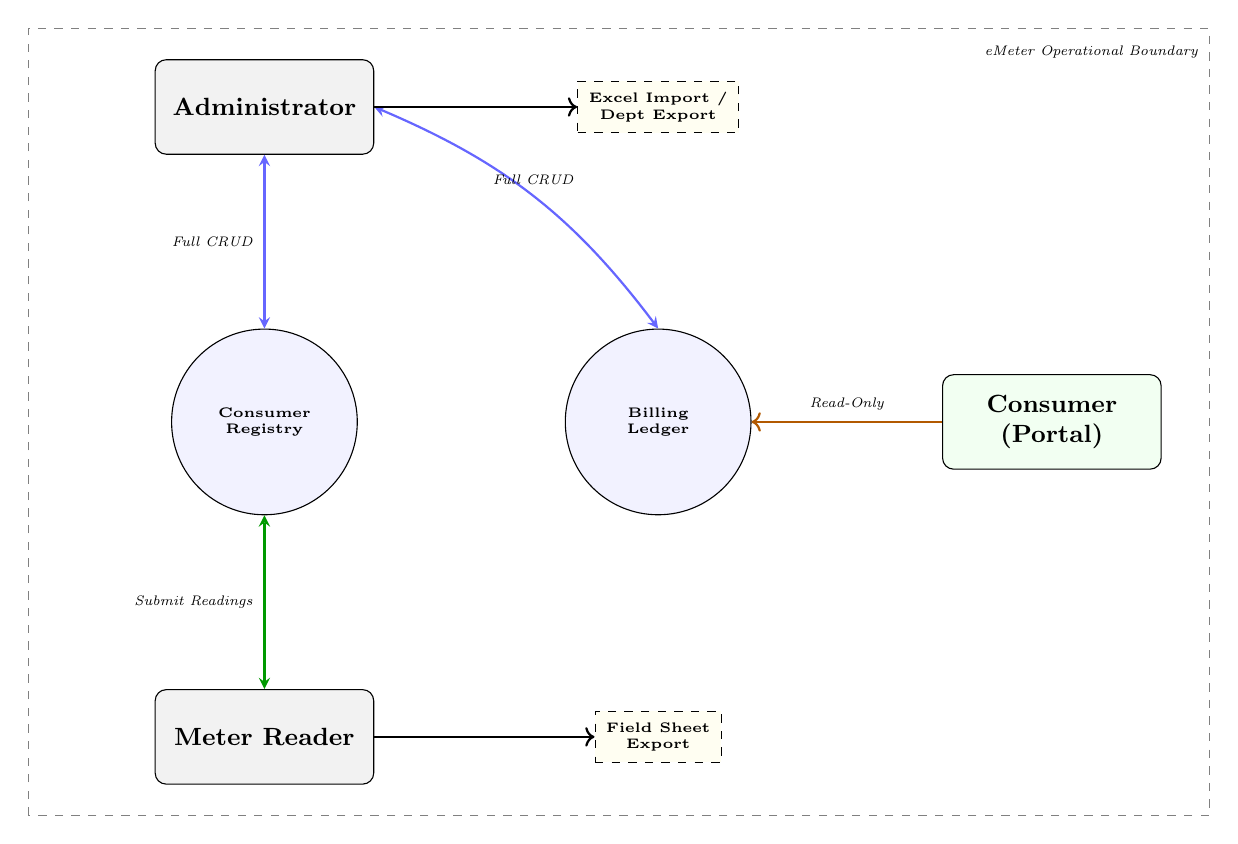
\begin{tikzpicture}[
        node distance=3cm,
        actor/.style={rectangle, draw, fill=gray!10, text width=2.5cm, align=center, minimum height=1.2cm, font={\small\bfseries}, rounded corners},
        entity/.style={circle, draw, fill=blue!5, text width=2cm, align=center, minimum size=2.2cm, font={\tiny\bfseries}},
        action/.style={draw, rectangle, fill=yellow!5, font=\tiny, inner sep=4pt, dashed, align=center},
        arrow/.style={thick, <->, >=stealth}
    ]
        % Core Entities
        \node (consumer) [entity] {Consumer \\ Registry};
        \node (bill) [entity, right of=consumer, xshift=2cm] {Billing \\ Ledger};

        % Actors
        \node (admin) [actor, above of=consumer, yshift=1cm] {Administrator};
        \node (reader) [actor, below of=consumer, yshift=-1cm] {Meter Reader};
        \node (portal) [actor, right of=bill, xshift=2cm, fill=green!5] {Consumer \\ (Portal)};

        % Shared CRUD Paths
        \draw [arrow, blue!60] (admin) -- node[left, font={\tiny\itshape}, text=black] {Full CRUD} (consumer);
        \draw [arrow, blue!60] (admin.east) to [bend left=15] node[above, font={\tiny\itshape}, text=black] {Full CRUD} (bill.north);

        \draw [arrow, green!60!black] (reader) -- node[left, font={\tiny\itshape}, text=black] {Submit Readings} (consumer);

        % Consumer portal read-only
        \draw [->, thick, orange!70!black] (portal.west) -- node[above, font={\tiny\itshape}, text=black] {Read-Only} (bill.east);

        % Specialized Workflows
        \node (exAdmin) [action, right of=admin, xshift=2cm] {\textbf{Excel Import /} \\ \textbf{Dept Export}};
        \node (exReader) [action, right of=reader, xshift=2cm] {\textbf{Field Sheet} \\ \textbf{Export}};

        \draw [->, thick] (admin) -- (exAdmin);
        \draw [->, thick] (reader) -- (exReader);

        % Background logic box
        \draw[dashed, gray] (-3, -5) rectangle (12, 5);
        \node at (10.5, 4.7) [font={\tiny\itshape}] {eMeter Operational Boundary};

    \end{tikzpicture}
    \caption{Functional Role-Interaction Model: Three-Actor System}
    \label{fig:role_model}
\end{figure}

\section{eMeter Retrieval Pipeline}
The eMeter retrieval pipeline defines the flow of utility data from physical ingestion at the meter level to its persistence and retrieval in the administrative dashboard. Figure \ref{fig:retrieval_pipeline} illustrates the sequential transition of data through the system's architectural layers.

\begin{figure}[htbp]
    \centering
    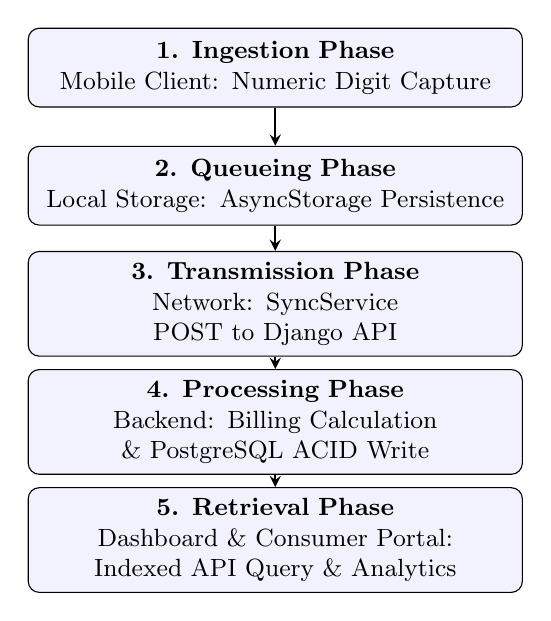
\begin{tikzpicture}[
        node distance=1.5cm,
        box/.style={rectangle, draw, fill=blue!5, text width=6cm, align=center, rounded corners, minimum height=1cm, font=\small},
        arrow/.style={thick, ->, >=stealth}
    ]
        \node (p1) [box] {\textbf{1. Ingestion Phase} \\ Mobile Client: Numeric Digit Capture};
        \node (p2) [box, below of=p1] {\textbf{2. Queueing Phase} \\ Local Storage: AsyncStorage Persistence};
        \node (p3) [box, below of=p2] {\textbf{3. Transmission Phase} \\ Network: SyncService POST to Django API};
        \node (p4) [box, below of=p3] {\textbf{4. Processing Phase} \\ Backend: Billing Calculation \& PostgreSQL ACID Write};
        \node (p5) [box, below of=p4] {\textbf{5. Retrieval Phase} \\ Dashboard \& Consumer Portal: Indexed API Query \& Analytics};

        \draw [arrow] (p1) -- (p2);
        \draw [arrow] (p2) -- (p3);
        \draw [arrow] (p3) -- (p4);
        \draw [arrow] (p4) -- (p5);
    \end{tikzpicture}
    \caption{eMeter Data Retrieval and Persistence Pipeline}
    \label{fig:retrieval_pipeline}
\end{figure}
\begin{enumerate}
    \item \textbf{Ingestion Phase}: Meter readers capture physical consumption digits via the mobile client's numeric input form.
    \item \textbf{Queueing Phase}: Data is stored in the \texttt{AsyncStorage} local queue if the network is unavailable.
    \item \textbf{Transmission Phase}: The SyncService dispatches a POST request to the Django \texttt{/api/readings/} endpoint.
    \item \textbf{Processing Phase}: The backend validates the reading against historical records, computes the consumption differential, applies the active billing policy, and stores the resulting reading and bill records atomically in PostgreSQL.
    \item \textbf{Retrieval Phase}: Administrators query the data through filtered API views, and consumers access their personal records via the consumer portal API.
\end{enumerate}

\section{Data Flow Diagrams}
Data Flow Diagrams (DFD) provide a graphical representation of the ``flow'' of data through eMeter, identifying the processes, external entities, and data stores involved.

\subsection{Level 0: Context Diagram}
The Context Diagram represents the system as a single process interacting with external entities. It illustrates the high-level boundary of eMeter, where Meter Readers provide readings and receive sync confirmations, Administrators provide configuration policies and receive analytical reports, and Consumers receive billing information.

\begin{figure}[htbp]
    \centering
    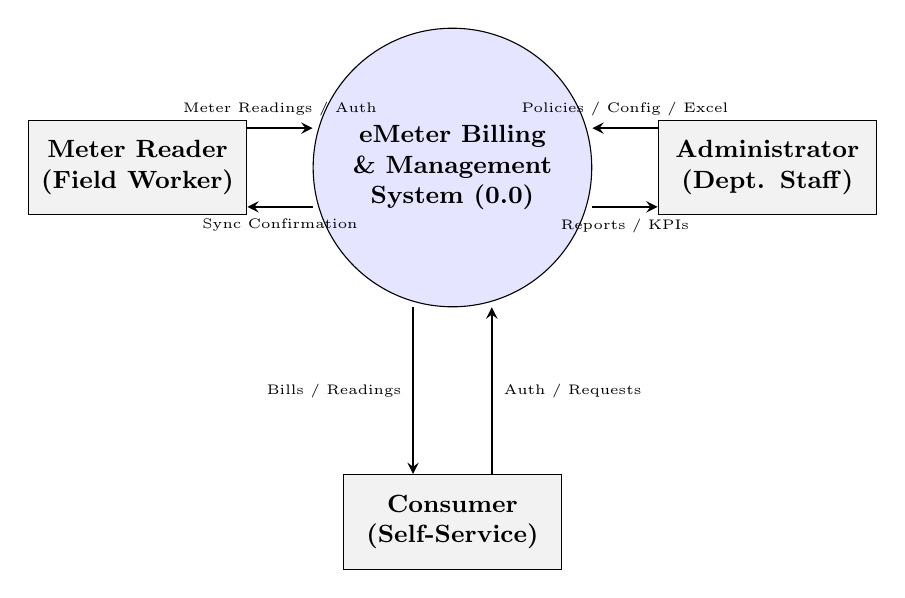
\begin{tikzpicture}[
        node distance=4cm,
        process/.style={circle, draw, fill=blue!10, text width=3cm, align=center, minimum size=3cm, font={\small\bfseries}},
        entity/.style={rectangle, draw, fill=gray!10, text width=2.5cm, align=center, minimum height=1.2cm, font={\small\bfseries}},
        arrow/.style={thick, ->, >=stealth}
    ]
        % System Process
        \node (system) [process] {eMeter Billing \\ \& Management \\ System (0.0)};
        
        % Entities
        \node (reader) [entity, left of=system] {Meter Reader \\ (Field Worker)};
        \node (admin) [entity, right of=system] {Administrator \\ (Dept. Staff)};
        \node (consumerE) [entity, below of=system, yshift=-0.5cm] {Consumer \\ (Self-Service)};

        % Flows for Reader
        \draw [arrow] ([yshift=0.5cm]reader.east) -- node[above, font=\tiny] {Meter Readings / Auth} ([yshift=0.5cm]system.west);
        \draw [arrow] ([yshift=-0.5cm]system.west) -- node[below, font=\tiny] {Sync Confirmation} ([yshift=-0.5cm]reader.east);

        % Flows for Admin
        \draw [arrow] ([yshift=0.5cm]admin.west) -- node[above, font=\tiny] {Policies / Config / Excel} ([yshift=0.5cm]system.east);
        \draw [arrow] ([yshift=-0.5cm]system.east) -- node[below, font=\tiny] {Reports / KPIs} ([yshift=-0.5cm]admin.west);

        % Flows for Consumer
        \draw [arrow] ([xshift=0.5cm]consumerE.north) -- node[right, font=\tiny] {Auth / Requests} ([xshift=0.5cm]system.south);
        \draw [arrow] ([xshift=-0.5cm]system.south) -- node[left, font=\tiny] {Bills / Readings} ([xshift=-0.5cm]consumerE.north);
    \end{tikzpicture}
    \caption{Level 0: Context Diagram of eMeter}
    \label{fig:dfd_level0}
\end{figure}

\begin{figure}[htbp]
    \centering
    \resizebox{\textwidth}{!}{
    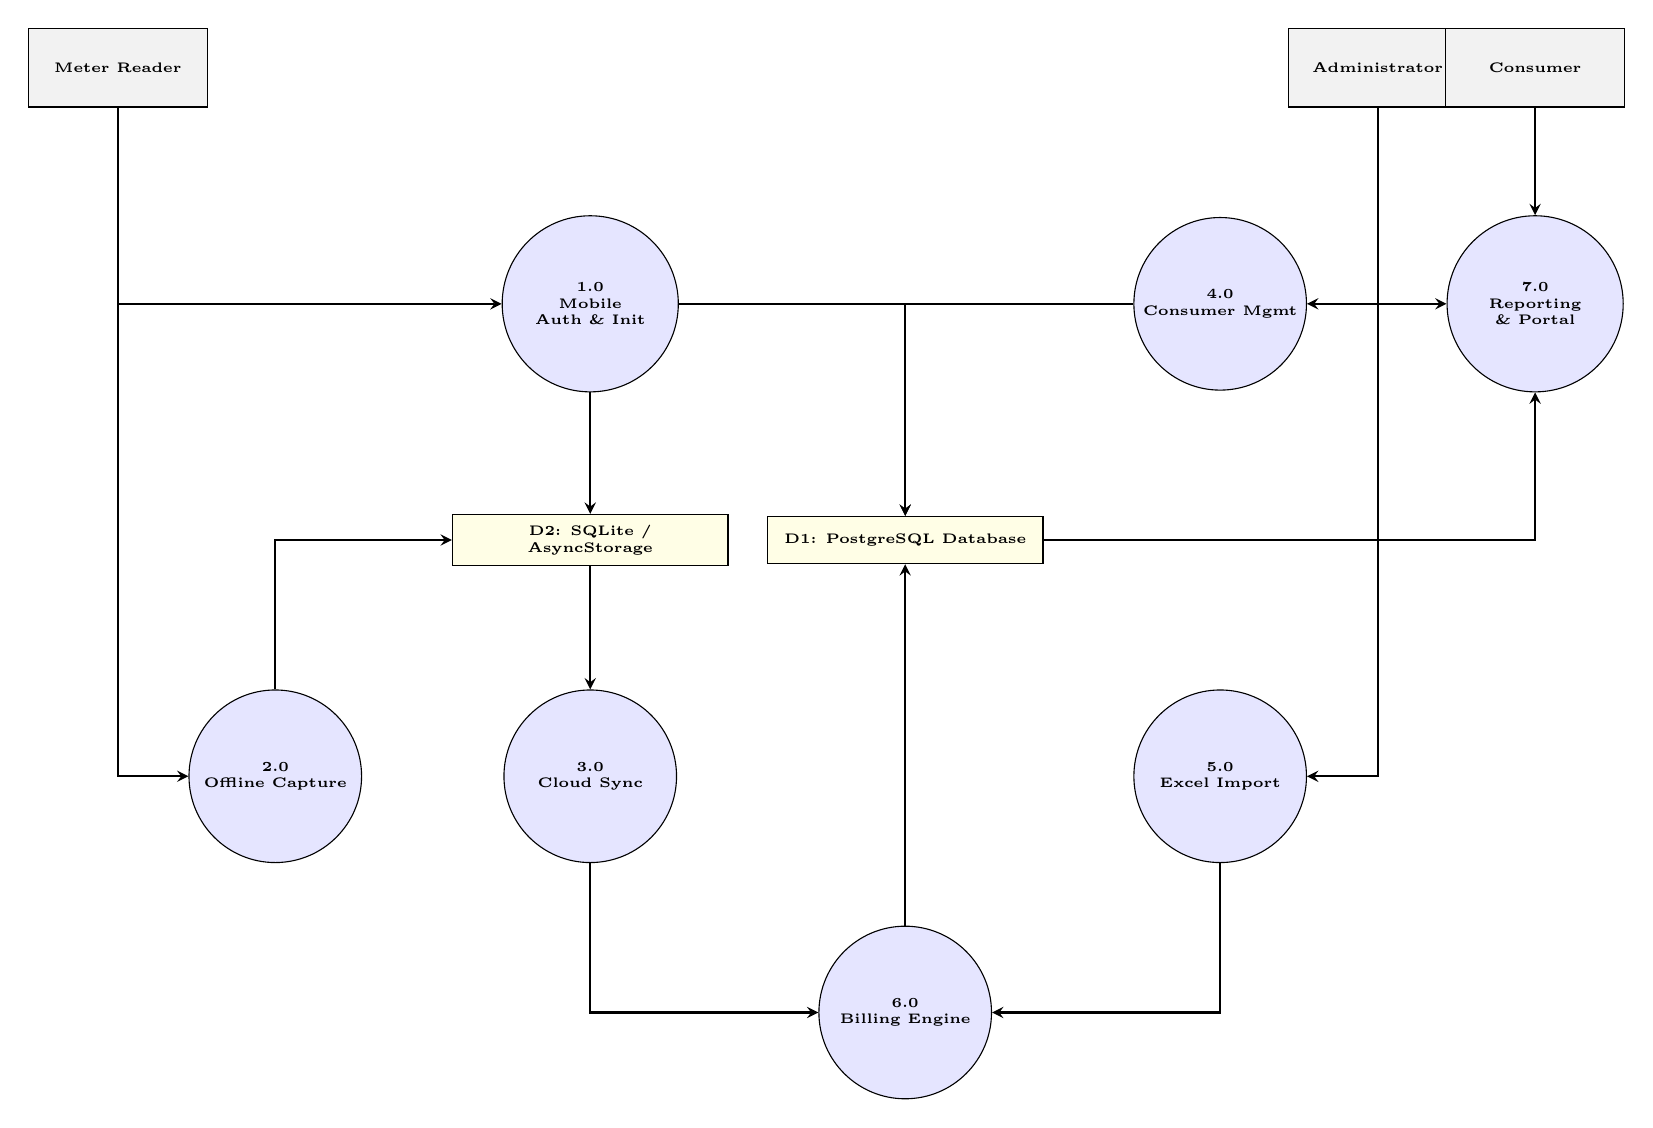
\begin{tikzpicture}[
        process/.style={circle, draw, fill=blue!10, text width=2cm, align=center, font={\tiny\bfseries}, inner sep=2pt},
        entity/.style={rectangle, draw, fill=gray!10, text width=2cm, align=center, minimum height=1cm, font={\tiny\bfseries}},
        datastore/.style={rectangle, draw, fill=yellow!10, minimum width=3.5cm, minimum height=0.6cm, font={\tiny\bfseries}, align=center},
        arrow/.style={thick, ->, >=stealth}
    ]
        % Entities (Top Row)
        \node (reader) [entity] at (0, 0) {Meter Reader};
        \node (admin) [entity] at (16, 0) {Administrator};
        \node (consumer) [entity] at (18, 0) {Consumer};

        % Left Column (Mobile / Offline)
        \node (p0) [process] at (6, -3) {1.0 \\ Mobile Auth \& Init};
        \node (db_local) [datastore] at (6, -6) {D2: SQLite / \\ AsyncStorage};
        \node (p1) [process] at (2, -9) {2.0 \\ Offline Capture};
        \node (p3) [process] at (6, -9) {3.0 \\ Cloud Sync};

        % Center (Core Backend)
        \node (db_cloud) [datastore] at (10, -6) {D1: PostgreSQL Database};
        \node (p4) [process] at (10, -12) {6.0 \\ Billing Engine};

        % Right Column (Admin & Portal)
        \node (p2) [process] at (14, -3) {4.0 \\ Consumer Mgmt};
        \node (p5) [process] at (14, -9) {5.0 \\ Excel Import};
        \node (p6) [process] at (18, -3) {7.0 \\ Reporting \& Portal};

        % Flows - Mobile
        \draw [arrow] (reader) |- (p0);
        \draw [arrow] (reader) |- (p1);
        \draw [arrow] (p0) -- (db_local);
        \draw [arrow] (p1) |- (db_local);
        \draw [arrow] (p0) -| (db_cloud);
        \draw [arrow] (db_local) -- (p3);
        \draw [arrow] (p3) |- (p4);

        % Flows - Admin
        \draw [arrow] (admin) |- (p2);
        \draw [arrow] (admin) |- (p5);
        \draw [arrow] (admin) |- (p6);
        
        % Flows - Consumer
        \draw [arrow] (consumer) -- (p6);

        % Flows - Internal & DB
        \draw [arrow] (p2) -| (db_cloud);
        \draw [arrow] (p5) |- (p4);
        \draw [arrow] (p4) -- (db_cloud);
        \draw [arrow] (db_cloud) -| (p6);
    \end{tikzpicture}
    }
    \caption{Level 1: Data Flow Diagram of eMeter (Strict Orthogonal Layout)}
    \label{fig:dfd_level1}
\end{figure}

\subsection{Level 1: Data Flow Diagram}
The Level 1 DFD decomposes the system into major functional processes:
\begin{itemize}
    \item \textbf{Process 1.0 (Authentication)}: Validates credentials and issues JWT tokens for all three actor types.
    \item \textbf{Process 2.0 (Consumer Management)}: Handles the lifecycle of consumer records.
    \item \textbf{Process 3.0 (Meter Reading \& Sync)}: Manages the transition of readings from mobile to database.
    \item \textbf{Process 4.0 (Billing Engine)}: Executes the calculation logic based on tariff settings and generates bills.
    \item \textbf{Process 5.0 (Excel Import)}: Processes batch reading uploads and triggers bulk bill generation.
    \item \textbf{Process 6.0 (Reporting \& Consumer Portal)}: Generates PDFs, Excel workbooks, and serves consumer self-service API endpoints.
\end{itemize}




\section{Database Design and Entity-Relationship Model}

The database structure was designed using relational modeling principles to ensure data consistency, integrity, and efficient querying.


\subsection{Entity-Relationship Diagram (ERD)}
The ERD maps the logical connections between the core system entities. Each entity is designed to store a specific set of attributes, with relationships defined to maintain referential integrity across the utility lifecycle.

\begin{figure}[htbp]
    \centering
    \begin{tikzpicture}[
        entity/.style={rectangle, draw, fill=blue!5, text width=2.8cm, align=center, minimum height=1.2cm, font={\tiny\bfseries}},
        relationship/.style={diamond, draw, fill=gray!10, text width=0.8.5cm, align=center, font=\tiny, aspect=1.5},
        arrow/.style={thick, -}
    ]
        % Entities with Key Attributes
        \node (consumer) [entity] at (0, 0) {Consumer \\ \rule{2.6cm}{0.4pt} \\ \tiny PK: id \\ consumer\_number (UQ)};
        \node (reading) [entity] at (7, 0) {MeterReading \\ \rule{2.6cm}{0.4pt} \\ \tiny PK: id \\ FK: consumer\_id};
        \node (bill) [entity] at (7, -4) {Bill \\ \rule{2.6cm}{0.4pt} \\ \tiny PK: id \\ FK: reading\_id};
        \node (settings) [entity] at (0, -4) {BillingSettings \\ \rule{2.6cm}{0.4pt} \\ \tiny PK: id};
        \node (user) [entity] at (7, 4) {User \\ \rule{2.6cm}{0.4pt} \\ \tiny PK: id \\ role: Admin/Reader};

        % Relationships
        \node (rel1) [relationship] at (3.5, 0) {has};
        \node (rel2) [relationship] at (7, -2) {triggers};
        \node (rel4) [relationship] at (3.5, -4) {governs};
        \node (rel5) [relationship] at (7, 2) {submits};

        % Connections with Cardinality
        \draw [arrow] (consumer) -- (rel1) node[midway, above] {1};
        \draw [arrow] (rel1) -- (reading) node[midway, above] {N};

        \draw [arrow] (reading) -- (rel2) node[midway, right] {1};
        \draw [arrow] (rel2) -- (bill) node[midway, right] {1};

        \draw [arrow] (settings) -- (rel4) node[midway, above] {1};
        \draw [arrow] (rel4) -- (bill) node[midway, above] {N};

        \draw [arrow] (user) -- (rel5);
        \draw [arrow] (rel5) -- (reading);
    \end{tikzpicture}
    \caption{Entity-Relationship Diagram (ERD) of eMeter System}
    \label{fig:erd}
\end{figure}

\subsection{Detailed Schema and Data Dictionary}
To ensure a robust and scalable implementation, eMeter utilizes a structured data dictionary defining the properties and constraints of each entity.

\subsubsection{Consumer Entity Schema}
The \texttt{Consumer} table is the primary registry for utility users. It enforces global uniqueness through a \texttt{consumer\_number} constraint and captures all information required for billing calculation, including the sanctioned load and connection phase.

\begin{table}[htbp]
\centering
\caption{Consumer Table Description}
\resizebox{\textwidth}{!}{
\begin{tabular}{|l|l|l|p{6cm}|}
\hline
\textbf{Field Name} & \textbf{Type} & \textbf{Constraints} & \textbf{Description} \\
\hline
id & INTEGER & PRIMARY KEY, AUTO & System-generated unique identifier \\ \hline
consumer\_number & VARCHAR(50) & UNIQUE, NOT NULL & Unique consumer registration identifier (e.g., CN001234) \\ \hline
name & VARCHAR(255) & NOT NULL & Full name of the electricity consumer \\ \hline
phone & VARCHAR(20) & NULLABLE & Consumer contact number \\ \hline
address & TEXT & NULLABLE & Residential or office address \\ \hline
post & VARCHAR(100) & NULLABLE & Designation or post (e.g., Professor, Clerk) \\ \hline
department & VARCHAR(100) & NULLABLE & Organizational department (e.g., Computer Science) \\ \hline
meter\_number & VARCHAR(100) & UNIQUE, NOT NULL & Physical electricity meter serial number \\ \hline
load\_kw & INTEGER & NOT NULL, DEFAULT 1 & Sanctioned load in kilowatts (1--5 KW) \\ \hline
billing\_type & VARCHAR(20) & NOT NULL & Account category: Salary or Non-Salary \\ \hline
connection\_type & VARCHAR(20) & NOT NULL & Meter phase: Single Phase or Three Phase \\ \hline
status & VARCHAR(20) & NOT NULL, DEFAULT Active & Connection status: Active, Inactive, or Suspended \\ \hline
initial\_reading & DECIMAL(10,2) & DEFAULT 0 & Starting meter value when connection was first registered \\ \hline
\end{tabular}
}
\label{tab:consumer_table}
\end{table}

\subsubsection{MeterReading Entity Schema}
This entity captures the physical consumption data submitted by field workers, both in online and offline-sync scenarios.

\begin{table}[htbp]
\centering
\caption{MeterReading Table Description}
\resizebox{\textwidth}{!}{
\begin{tabular}{|l|l|l|p{6cm}|}
\hline
\textbf{Field Name} & \textbf{Type} & \textbf{Constraints} & \textbf{Description} \\
\hline
id & INTEGER & PRIMARY KEY, AUTO & Unique identifier for the meter reading record \\ \hline
consumer & INTEGER & FOREIGN KEY, NOT NULL & References Consumer entity (ON DELETE PROTECT) \\ \hline
reader & INTEGER & FOREIGN KEY, NULLABLE & References User who submitted the reading \\ \hline
previous\_reading & DECIMAL(10,2) & NOT NULL & Previously recorded meter value (kWh) \\ \hline
current\_reading & DECIMAL(10,2) & NOT NULL & Current meter value entered by the field reader (kWh) \\ \hline
units & DECIMAL(10,2) & GENERATED & Consumption differential (current minus previous) \\ \hline
reading\_date & DATE & NOT NULL & Date on which the reading was taken \\ \hline
remarks & TEXT & NULLABLE & Optional field notes from the meter reader \\ \hline
\end{tabular}
}
\label{tab:meterreading_table}
\end{table}

\subsubsection{Bill Entity Schema}
The \texttt{Bill} entity is the result of the automated calculation service. It represents the financial liability of the consumer and carries a complete charge breakdown as well as a snapshot of the consumer details at the time of billing.

\begin{table}[H]
\centering
\caption{Bill Table Description}
\resizebox{\textwidth}{!}{
\begin{tabular}{|l|l|l|p{6cm}|}
\hline
\textbf{Field Name} & \textbf{Type} & \textbf{Constraints} & \textbf{Description} \\
\hline
id & INTEGER & PRIMARY KEY, AUTO & Unique identifier for the generated bill \\ \hline
bill\_number & VARCHAR(50) & UNIQUE, NOT NULL & Human-readable bill reference (e.g., BILL-001) \\ \hline
reading & INTEGER & FOREIGN KEY, NOT NULL & References the MeterReading that triggered this bill \\ \hline
consumer\_name & VARCHAR(255) & NOT NULL & Snapshot of consumer name at billing time \\ \hline
consumer\_number & VARCHAR(50) & NOT NULL & Snapshot of consumer number at billing time \\ \hline
meter\_number & VARCHAR(100) & NOT NULL & Snapshot of meter number at billing time \\ \hline
billing\_period & VARCHAR(20) & NOT NULL & Month and year of the bill (e.g., Jul-26) \\ \hline
units & DECIMAL(10,2) & NOT NULL & Units consumed (kWh) \\ \hline
rate\_per\_unit & DECIMAL(10,4) & NOT NULL & Energy rate (Rs./kWh) used for this bill \\ \hline
energy\_charges & DECIMAL(10,2) & NOT NULL & Charge for consumed units (units x rate) \\ \hline
fixed\_charges & DECIMAL(10,2) & NOT NULL & Fixed charge based on sanctioned load (load\_kw x fixed\_charge\_per\_kw) \\ \hline
duty\_charge & DECIMAL(10,2) & NOT NULL & Electricity duty applied as a percentage \\ \hline
meter\_rent & DECIMAL(10,2) & NOT NULL & Monthly meter rental (varies by phase) \\ \hline
regulatory\_surcharge & DECIMAL(10,2) & NOT NULL & Regulatory surcharge component \\ \hline
arrears & DECIMAL(10,2) & DEFAULT 0 & Outstanding amount from a previous unpaid bill \\ \hline
late\_payment\_surcharge & DECIMAL(10,2) & DEFAULT 0 & Penalty applied when bill is overdue \\ \hline
total\_amount & DECIMAL(10,2) & NOT NULL & Grand total of all charge components \\ \hline
is\_paid & BOOLEAN & DEFAULT FALSE & Payment completion status \\ \hline
bill\_date & DATE & NOT NULL & Date on which the bill was generated \\ \hline
due\_date & DATE & NOT NULL & Payment deadline date \\ \hline
\end{tabular}
}
\label{tab:bill_table}
\end{table}

\subsubsection{Billing Settings Entity Schema}
This entity defines the global tariff policies used by the billing calculation engine. It uses a flat-rate model where a single per-unit energy rate is combined with fixed charges based on sanctioned load and phase-specific meter rents.

\begin{table}[htbp]
\centering
\caption{Billing Settings Table Description}
\resizebox{\textwidth}{!}{
\begin{tabular}{|l|l|l|p{6cm}|}
\hline
\textbf{Field Name} & \textbf{Type} & \textbf{Constraints} & \textbf{Description} \\
\hline
id & INTEGER & PRIMARY KEY, AUTO & Unique identifier for the billing configuration record \\ \hline
unit\_rate & DECIMAL(10,4) & NOT NULL & Price per kWh of consumed electricity (e.g., Rs. 8.56) \\ \hline
tax\_pct & DECIMAL(5,2) & NOT NULL & Electricity duty percentage applied on energy charges (e.g., 7.5\%) \\ \hline
fixed\_charge\_per\_kw & DECIMAL(10,2) & NOT NULL & Monthly fixed connection charge per KW of sanctioned load (e.g., Rs. 400) \\ \hline
meter\_rent\_1ph & DECIMAL(10,2) & NOT NULL & Monthly meter rental fee for single-phase meters (e.g., Rs. 10) \\ \hline
meter\_rent\_3ph & DECIMAL(10,2) & NOT NULL & Monthly meter rental fee for three-phase meters (e.g., Rs. 25) \\ \hline
created\_at & DATETIME & AUTO & Timestamp when the configuration was saved \\ \hline
\end{tabular}
}
\label{tab:billingsettings_table}
\end{table}

\subsection{Integrity Constraints and Normalization}
The eMeter database is strictly normalized to the \textbf{Third Normal Form (3NF)} to eliminate update anomalies and data redundancy.

\subsubsection{Referential Integrity}
The system implements \texttt{ON DELETE PROTECT} on core relationships. For instance, a \texttt{Consumer} record cannot be purged if it is referenced by existing \texttt{Bill} records. This ensures that historical financial audits remain consistent and untampered.

\subsubsection{Policy Snapshotting}
One of the most critical design decisions in eMeter is \textbf{Policy Snapshotting}. Rather than linking each bill to a \texttt{BillingSettings} foreign key (which could change), the billing engine snapshots the exact rate values (unit rate, duty percentage, meter rent, etc.) directly into the \texttt{Bill} record's \texttt{rate\_per\_unit} and charge fields at the time of generation. This ensures that even if rates are updated in the future, past bills remain mathematically valid and auditable according to the policy that was active at the time of their creation.

\subsection{Indexes and Performance Optimization}
As the consumer base grows, query performance becomes a critical bottleneck. The eMeter schema utilizes B-Tree indexing on frequently queried columns:
\begin{itemize}
    \item \textbf{consumer\_number Index}: Facilitates instantaneous lookup in the mobile client and consumer portal.
    \item \textbf{is\_paid Index}: Optimizes administrative dashboard queries for revenue reports.
    \item \textbf{reading\_date / bill\_date Index}: Ensures that historical consumption trends and billing period filters are rendered without latency.
\end{itemize}

\subsection{Local Mobile Persistence Schema (Offline Queue)}
A significant architectural contribution of the eMeter ecosystem is its fault-tolerant offline data capture. While the centralized PostgreSQL database serves as the ultimate source of truth, the React Native mobile application employs a local database strategy (utilizing SQLite or AsyncStorage) to temporarily persist data on the field worker's device. 

The mobile schema consists of two primary local data structures:

\subsubsection{Local Consumer Cache}
To enable meter readers to search for and identify consumer meters in zero-connectivity areas, a heavily optimized subset of the consumer dataset is cached on the device during the morning sync.
\begin{itemize}
    \item \textbf{\texttt{id}}: The primary key representing the consumer ID on the remote database.
    \item \textbf{\texttt{consumer\_number}}: Indexed locally for rapid, sub-millisecond search retrieval without network calls.
    \item \textbf{\texttt{name} \& \texttt{address}}: Used for visual verification by the meter reader at the premises.
    \item \textbf{\texttt{last\_reading}}: Cached to allow the mobile UI to enforce logical boundaries (e.g., preventing the reader from entering a current reading lower than the previous reading).
\end{itemize}

\subsubsection{Offline Reading Queue}
When a meter reader submits a reading while offline, it is serialized as a JSON object and pushed to a robust local queue. This ensures zero data loss and allows the reader to continue working without interruption.
\begin{itemize}
    \item \textbf{\texttt{uuid}}: A locally generated unique identifier for the transaction to prevent duplicate submissions upon syncing.
    \item \textbf{\texttt{consumer\_id}}: Foreign key referencing the local consumer cache.
    \item \textbf{\texttt{current\_reading}}: The actual reading value captured from the meter.
    \item \textbf{\texttt{reading\_date}}: The exact timestamp of the capture, ensuring billing accuracy regardless of when the network is restored.
    \item \textbf{\texttt{sync\_status}}: A crucial state flag (\texttt{'pending'}, \texttt{'syncing'}, \texttt{'synced'}, or \texttt{'failed'}) that dictates the behavior of the background synchronization daemon.
\end{itemize}

\newpage

\section{UML Structural Models}
The structural model of eMeter provides a static view of the system, identifying the key entities, their internal structures, and the relationships that govern their interactions.

\subsection{Use Case Diagram}
The Use Case diagram identifies the interactions between actors and the system. It serves as a high-level representation of the functional requirements, illustrating the operational boundaries between the Administrator, Meter Reader, and Consumer actors. The diagram encapsulates core functionalities such as role-based authentication, consumer management, automated bill calculation, Excel bulk import, and consumer self-service portal access.

% \begin{figure}[htbp]
%     \centering
%     \includegraphics[width=0.8\textwidth, height=0.4\textheight, keepaspectratio]{{USE_CASE_eMeter.png}}
%     \caption{UML Use Case Diagram: Role-Based Interactions}
%     \label{fig:use_case}
% \end{figure}

\subsection{Use Case Diagram}
The Use Case diagram identifies the interactions between actors and the system. It serves as a high-level representation of the functional requirements, illustrating the operational boundaries between the Administrator, Meter Reader, and Consumer actors. The diagram encapsulates core functionalities such as role-based authentication, consumer management, automated bill calculation, Excel bulk import, and consumer self-service portal access.

\subsection{Use Case Diagram}
The Use Case diagram identifies the interactions between actors and the system. It serves as a high-level representation of the functional requirements, illustrating the operational boundaries between the Administrator, Meter Reader, and Consumer actors. The diagram encapsulates core functionalities such as role-based authentication, consumer management, automated bill calculation, Excel bulk import, and consumer self-service portal access.

\begin{figure}[htbp]
    \centering
    \includegraphics[width=0.75\linewidth]{UML_eMeter.png}
    \caption{UML Class Diagram for eMeter Backend Architecture}
    \label{fig:class_diagram}
\end{figure}

\begin{figure}
    \centering
    \includegraphics[width=1.25\linewidth, angle = 270]{eMeter-USECASE.drawio.png}
    \caption{Well Detailed Use Case Diagram For Admin and Field Reader}
    \label{fig:placeholder}
\end{figure}

\begin{figure}[htbp]
    \centering
    \resizebox{\textwidth}{!}{
    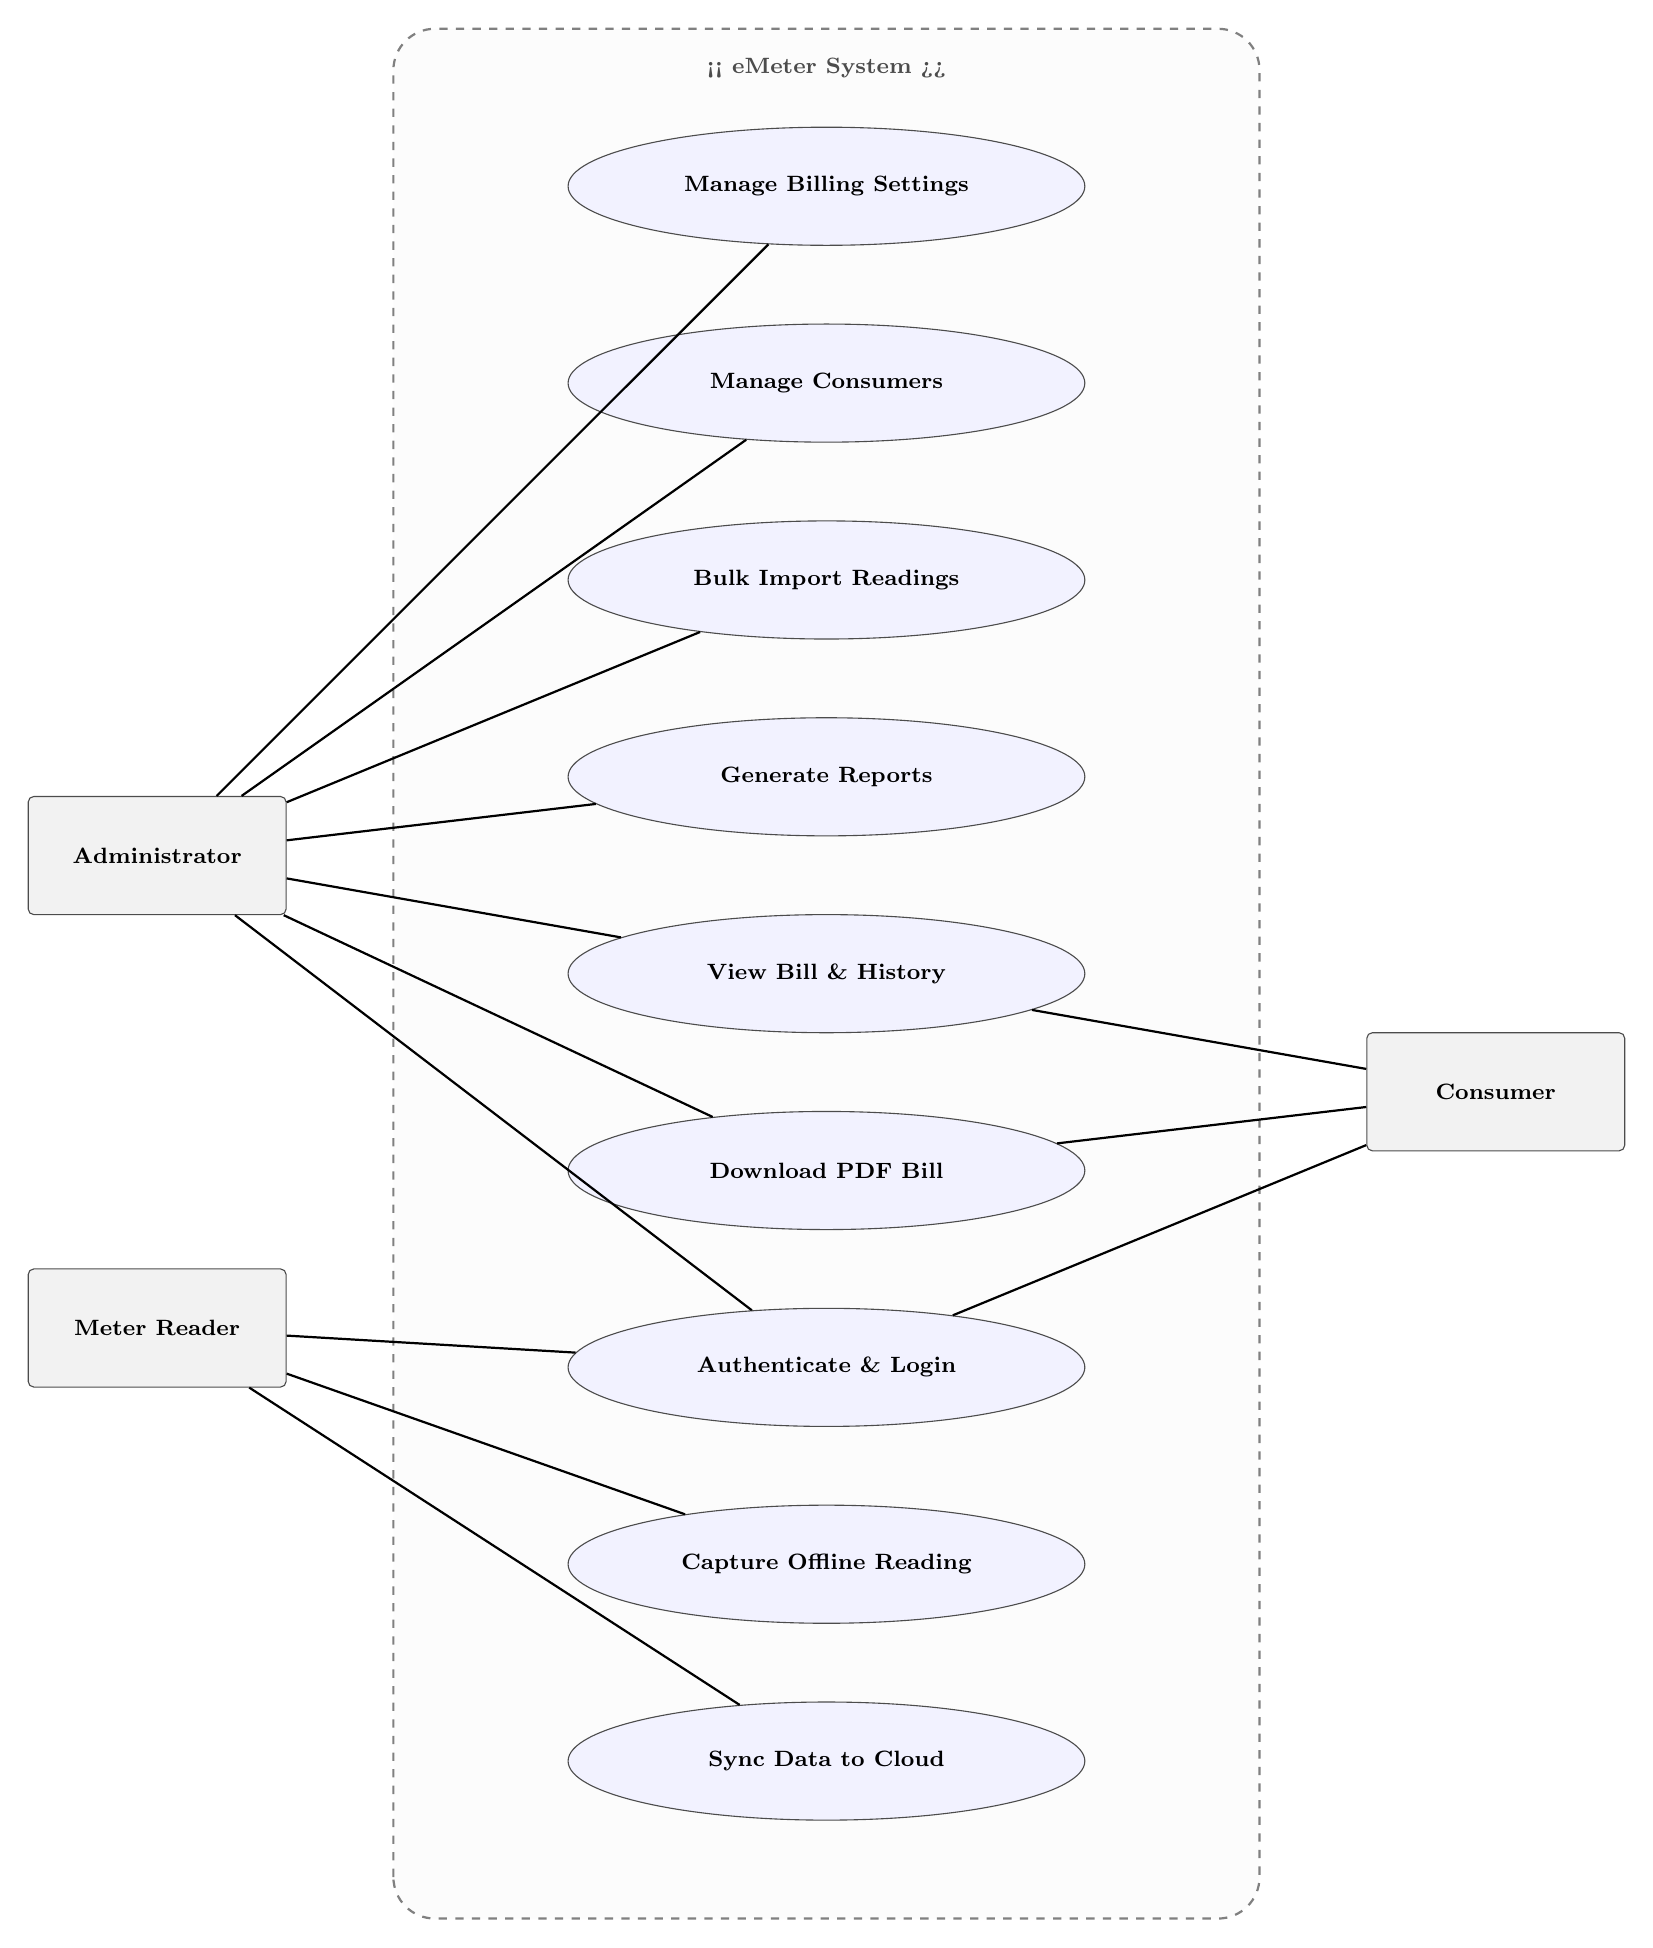
\begin{tikzpicture}[
        usecase/.style={ellipse, draw=black!70, fill=blue!5, text width=4.5cm, align=center, font={\footnotesize\bfseries}, minimum height=1.5cm, inner sep=2pt},
        actor/.style={rectangle, draw=black!70, fill=gray!10, text width=3cm, align=center, minimum height=1.5cm, font={\footnotesize\bfseries}, rounded corners=2pt},
        line/.style={thick, -}
    ]
        % System Boundary
        \draw[thick, draw=black!50, fill=gray!2, rounded corners=15pt, dashed] (-5.5, -12) rectangle (5.5, 12);
        \node[font={\footnotesize\bfseries}, text=black!70] at (0, 11.5) {<< eMeter System >>};
        % Actors
        \node (admin) [actor] at (-8.5, 1.5) {Administrator};
        \node (reader) [actor] at (-8.5, -4.5) {Meter Reader};
        \node (consumer) [actor] at (8.5, -1.5) {Consumer};
        % Use Cases
        \node (uc1) [usecase] at (0, 10) {Manage Billing Settings};
        \node (uc2) [usecase] at (0, 7.5) {Manage Consumers};
        \node (uc3) [usecase] at (0, 5) {Bulk Import Readings};
        \node (uc4) [usecase] at (0, 2.5) {Generate Reports};
        \node (uc6) [usecase] at (0, 0) {View Bill \& History};
        \node (uc7) [usecase] at (0, -2.5) {Download PDF Bill};
        \node (uc5) [usecase] at (0, -5) {Authenticate \& Login};
        \node (uc8) [usecase] at (0, -7.5) {Capture Offline Reading};
        \node (uc9) [usecase] at (0, -10) {Sync Data to Cloud};
        % Admin Lines
        \draw [line] (admin) -- (uc1);
        \draw [line] (admin) -- (uc2);
        \draw [line] (admin) -- (uc3);
        \draw [line] (admin) -- (uc4);
        \draw [line] (admin) -- (uc6);
        \draw [line] (admin) -- (uc7);    
        \draw [line] (admin) -- (uc5);
        % Reader Lines
        \draw [line] (reader) -- (uc5);
        \draw [line] (reader) -- (uc8);
        \draw [line] (reader) -- (uc9);
        % Consumer Lines
        \draw [line] (consumer) -- (uc6);
        \draw [line] (consumer) -- (uc7);
        \draw [line] (consumer) -- (uc5);
    \end{tikzpicture}
    }
    \caption{UML Use Case Diagram: Role-Based Interactions (Topologically Sorted Layout)}
    \label{fig:use_case}
\end{figure}


\subsection{Class Diagram}
The Class Diagram illustrates the static structure of the eMeter backend, defining the domain models and their logical associations. It details the attributes and methods of core classes including \texttt{Consumer}, \texttt{MeterReading}, \texttt{Bill}, \texttt{BillingSettings}, and \texttt{User}. The diagram models the ``one-to-many'' relationship between Consumers and their historical Readings, as well as the ``one-to-one'' link between a specific Reading event and its corresponding generated Bill.



\newpage

\section{Behavioral Model (Sequence Diagram)}
The Sequence Diagram models the dynamic collaboration between objects over time. The following diagram illustrates the ``Reading Synchronization'' sequence, identifying the chronological flow of messages between the mobile client, backend services, and the data layer.
\begin{figure}
    \centering
    \includegraphics[width=1.5\linewidth, angle = 270]{sequence_UML.png}
    \caption{Detailed Sequence Diagram}
    \label{fig:placeholder}
\end{figure}

% \begin{figure}[htbp]
%     \centering
%     \begin{tikzpicture}[font=\small]
%         % Lifelines (x-spacing widened from 3/6 to 5/10)
%         \draw[dashed] (0,0) -- (0,-10) node[below] {Mobile Client};
%         \draw[dashed] (5,0) -- (5,-10) node[below] {Django API};
%         \draw[dashed] (10,0) -- (10,-10) node[below] {PostgreSQL DB};
%         % Actors at top
%         \node[draw, fill=gray!10] at (0,0.5) {Meter Reader};
%         \node[draw, fill=blue!10] at (5,0.5) {Backend Server};
%         \node[draw, fill=yellow!10] at (10,0.5) {Database};
%         % Sequence (y-spacing widened, roughly 1.4x the original gaps)
%         \draw[->, >=stealth, thick] (0,-1.5) -- node[above] {POST /api/readings/ (Auth Header)} (5,-1.5);
%         \node at (5,-2.3) [anchor=west, xshift=0.15cm, draw, fill=blue!5, text width=2.4cm, align=center] {Validate Token \& Reading};
        
%         \draw[->, >=stealth, thick] (5,-3.7) -- node[above] {INSERT Reading Record} (10,-3.7);
%         \draw[<-, >=stealth, dashed, thick] (5,-4.4) -- node[above] {Success (ID)} (10,-4.4);
        
%         \node at (5,-5.7) [anchor=west, xshift=0.15cm, draw, fill=blue!5, text width=2.8cm, align=center] {Trigger Billing Algorithm};
        
%         \draw[->, >=stealth, thick] (5,-7.2) -- node[above] {INSERT Bill Record} (10,-7.2);
%         \draw[<-, >=stealth, dashed, thick] (5,-7.9) -- node[above] {Success} (10,-7.9);
        
%         \draw[<-, >=stealth, dashed, thick] (0,-9.3) -- node[above] {201 Created (Sync Complete)} (5,-9.3);
%     \end{tikzpicture}
%     \caption{UML Sequence Diagram: Meter Reading Synchronization Flow}
% \end{figure}

\subsection{State Diagram}
The State Diagram models the lifecycle of a meter reading record, from its initial capture on the mobile device to its final state as a finalized bill record on the central server.
\begin{figure}
    \centering
    \includegraphics[width=0.5\linewidth]{state_diagram_UML.png}
    \caption{Detailed State Diagram}
    \label{fig:placeholder}
\end{figure}


% \begin{figure}[htbp]
%     \centering
%     \begin{tikzpicture}[
%         node distance=4.5cm,
%         state/.style={circle, draw, thick, fill=blue!5, text width=2.2cm, align=center, font=\small, minimum size=2cm},
%         arrow/.style={thick, ->, >=stealth}
%     ]
%         % Start
%         \node (start) [circle, fill=black, inner sep=3pt] at (-2.5, 0) {};
        
%         % States
%         \node (pending)   [state] at (0,0) {Pending (Local AsyncStorage)};
%         \node (syncing)   [state, right of=pending] {Synchronizing (Network Active)};
%         \node (persisted) [state, right of=syncing] {Persisted (PostgreSQL)};
%         \node (billed)    [state, below of=persisted, yshift=1.5cm] {BillingActive (Policy Applied)};
%         \node (finalized) [state, below of=syncing, yshift=1.5cm] {Finalized (Notification Sent)};
        
%         % End marker
%         \node (end) [circle, draw, thick, inner sep=1pt] at ($(finalized) + (0,-2.6)$) {};
%         \node (endfill) [circle, fill=black, inner sep=1.5pt] at (end) {};
        
%         % Transitions
%         \draw [arrow] (start) -- (pending);
%         \draw [arrow] (pending) -- node[above, font=\small] {Sync Trigger} (syncing);
%         \draw [arrow] (syncing) -- node[above, font=\small] {API 201} (persisted);
%         \draw [arrow] (syncing) edge[bend left=25] node[below, font=\small] {Fail / Timeout} (pending);
%         \draw [arrow] (persisted) -- node[right, font=\small] {Atomic Trigger} (billed);
%         \draw [arrow] (billed) -- node[above, font=\small] {PDF Generated} (finalized);
%         \draw [arrow] (finalized) -- (end);
%     \end{tikzpicture}
%     \caption{UML State Diagram: Meter Reading Lifecycle}
% \end{figure}


\section{Design Tools and Architectural Limitations}

\subsection{Design Tools}
The system architecture and modeling were performed using:
\begin{itemize}
    \item \textbf{VS Code}: For core implementation and scripting.
    \item \textbf{Draw.io / Mermaid.js}: For DFD, ERD, and UML modeling.
    \item \textbf{Postman}: For API design and endpoint verification.
\end{itemize}

\subsection{Architectural Limitations}
\begin{itemize}
    \item \textbf{Memory Bound}: Large-scale analytical queries for millions of records may require additional caching layers (e.g., Redis).
    \item \textbf{Single-Server Billing}: The PDF generation using \textit{xhtml2pdf} is synchronous and CPU-bound; at very high concurrency, an asynchronous task queue (e.g., Celery with Redis) would be required.
\end{itemize}

\section{Module Design}

\subsection{Authentication Module}
This module handles user login, token generation, session validation, and role-based authorization. JWT tokens are issued upon successful authentication and are included in subsequent API requests. The consumer portal uses a separate authentication path (\texttt{/api/consumer/portal/login/}) with its own token scope to enforce complete isolation from the admin system.

\subsection{Consumer and User Management Module}
The management module enables administrators to maintain consumer records through full CRUD interfaces. Key operations include consumer registration (with automatic consumer number generation), status management (Active/Inactive/Suspended), and portal password resets. The module enforces referential integrity, preventing deletion of consumers with existing billing records.

\subsection{Meter Reading and Bill Management Module}
This module provides the core data lifecycle management. It accepts readings from both the mobile app (online and offline-sync) and the web dashboard (manual administrative entry). Upon receiving a valid reading, the module atomically creates the reading record and triggers the billing engine within a single database transaction.

\subsection{Excel Bulk Import Module}
This module handles the administrative workflow of uploading \texttt{.xlsx} or \texttt{.xls} files to generate bills in batch. The backend auto-detects the column layout (3-column: consumer number, reading, date; or 4-column: consumer number, meter number, reading, date), validates each row, creates readings, and generates bills. A structured result response reports successes, failures, and per-row error messages to the administrator.

\subsection{Consumer Self-Service Portal Module}
This module serves the consumer-facing API endpoints. It enforces strict data isolation, ensuring each authenticated consumer can only access their own reading history and bills. The module provides endpoints for listing readings, listing bills (with pagination), and a PDF bill download action that renders the bill HTML to a PDF using the same template as the administrative PDF generation.

\subsection{Billing and Excel Reporting Module}
The billing module automates invoice generation based on the active \texttt{BillingSettings} policy. The reporting engine handles multi-role Excel operations. Meter Readers can export the offline reading queue as a spreadsheet, while Administrators manage global bulk imports, download filtered billing reports, and export consumer data.

\subsection{Reporting Module}
The reporting module generates analytical summaries for the administrative dashboard, including monthly consumption bar charts, revenue breakdown donut charts (paid vs. unpaid), and a top-10 consumer ranking by total kWh usage.

\section{Security Mechanisms}
Security is a fundamental component of the proposed system architecture. All API communications are secured using HTTPS. JWT authentication is implemented to verify user identity, and role-based permissions ensure that users can only access relevant functionalities. Consumer portal tokens are scoped separately from admin/reader tokens to prevent privilege escalation.

\section{External Interface Requirements}
The external interfaces for eMeter are realized through three client applications: the React-based administrative web portal, the React-based consumer self-service portal, and the Expo-based mobile field application, all utilizing RESTful communication protocols with the Django backend.

\section{Summary}
This chapter detailed the structural and behavioral design of the eMeter platform. By defining the architecture, database schema, and data flow models, the design phase ensures that the subsequent implementation is built upon a robust and logically consistent framework.

\clearpage
\chapter{SYSTEM IMPLEMENTATION AND TESTING}

\section{System Requirements and Specifications}
The implementation required coordinating multiple tech stacks within a monorepo structure.

\subsection{Backend Implementation (Django)}
The backend APIs were constructed using Django REST Framework generic views and ViewSets. The billing algorithm was encapsulated within a transaction block (\texttt{transaction.atomic}) to ensure that a \texttt{MeterReading} and its corresponding \texttt{Bill} are either created together or fail together, preventing database anomalies. 

The PDF generation utilizes a client-side HTML template (\texttt{generateBillHtml}) that renders the complete bill invoice in the browser via a hidden iframe print mechanism, producing a print-ready document without server-side rendering overhead. Server-side PDF rendering via \textit{xhtml2pdf} is also available as an alternative pathway.

The Excel bulk import endpoint (\texttt{/api/billing/import-readings-excel/}) accepts multipart form data, parses the file using the \texttt{openpyxl} library, and processes each row sequentially. Errors are collected per-row and returned in a structured JSON response alongside successfully generated bills.

\subsection{Frontend Implementation (React \& TailwindCSS)}
The admin dashboard and consumer portal are both built using React 18 with TypeScript and \textbf{Vite} as the build tool. The application uses centralized API modules (\texttt{lib/api.ts} for admin, \texttt{contexts/ConsumerAuthContext.tsx} for the consumer portal) to manage all HTTP communication.

\texttt{TailwindCSS} was employed to rapidly build a responsive, utility-first UI. The \textbf{SheetJS (xlsx)} library handles client-side Excel template generation (for the bulk import template download) and result rendering.

The consumer portal is a distinct set of protected routes (\texttt{/consumer/*}) rendered within the same React application but completely isolated in authentication state from the administrative interface.

\subsection{Mobile Implementation (React Native \& Expo)}
The mobile app relies heavily on React Navigation for screen transitions. The offline queue was implemented by serializing reading objects into JSON strings and appending them to an array stored in \texttt{AsyncStorage}. The \textbf{NetInfo} API continuously monitors connection status. When online, a \texttt{pushOfflineQueueToServer} asynchronous function iterates over the queue, dispatching POST requests to the backend for each pending reading. The \textbf{expo-document-picker} library enables import of the \texttt{eMeter\_Offline\_Sync.json} file from the device filesystem for offline consumer registry initialization.

\section{Hardware Requirement}
\subsection{Server Environment}
\begin{itemize}
    \item \textbf{Processor}: Multi-core CPU (e.g., AWS EC2 t3.medium or higher) for handling concurrent API requests and PDF rendering tasks.
    \item \textbf{RAM}: 4GB Minimum (8GB Recommended).
    \item \textbf{Database Storage}: 50GB SSD, adequate for consumer records and billing history.
\end{itemize}

\subsection{Client Environment}
\begin{itemize}
    \item \textbf{Web (Admin \& Consumer Portal)}: Modern evergreen browser (Chrome, Safari, Firefox).
    \item \textbf{Mobile}: Android 8.0+ or iOS 13+ device.
\end{itemize}

\section{Software Requirement}
\begin{itemize}
    \item \textbf{Backend}: Python 3.10+, Django 4.x, PostgreSQL 16.
    \item \textbf{Frontend}: TypeScript, React 18, Vite, TailwindCSS.
    \item \textbf{Mobile}: Expo SDK 50+, React Native.
\end{itemize}

\section{System Testing}
Testing ensures the reliability of the critical billing algorithms.

\subsection{Unit Testing}
Python \texttt{unittest} was used to verify the billing engine. Mock readings were fed into the calculation function, and the output was asserted against manually calculated expected values to ensure rates, duty percentages, fixed charges, and meter rents were applied correctly. A dedicated test module (\texttt{test\_modules.py}) covers the core billing formula for both single-phase and three-phase consumers.

\subsection{Integration Testing}
The integration between the mobile app's offline queue and the Django backend was tested by simulating network drops in the Expo emulator. Readings taken while offline were verified to appear in the database only after the network was reconnected and the sync function fired. The Excel import endpoint was tested against the provided sample template (\texttt{test\_bot\_readings.xlsx}) to verify both the 3-column and 4-column layout detection.

\subsection{Performance Analysis}
The backend was tested for N+1 query problems. By utilizing Django's \texttt{select\_related} and \texttt{prefetch\_related} in the ORM, the API response times for listing thousands of consumers and their latest bills were reduced from over 2 seconds to under 200 milliseconds.

\chapter{APPLICATION AND SCOPE}

\section{Application Areas}
The eMeter platform is designed for immediate deployment in various utility management contexts:

\subsection{University Campuses and Institutional Settings}
Educational institutions such as Aligarh Muslim University, with large residential and departmental complexes, represent the primary target deployment. The system supports categorization of consumers by department and designation (post), enabling precise administrative tracking and reporting across institutional hierarchies.

\subsection{Municipal Electricity Boards}
Local government bodies can adopt the platform to modernize their existing grid management, replacing paper trails with a fully auditable digital database.

\subsection{Private Residential Complexes and Societies}
Large housing societies that purchase bulk electricity and redistribute it to residents via sub-meters can use eMeter to manage internal billing accurately and transparently.

\subsection{Adaptability to Other Utilities}
Due to the dynamic nature of the \texttt{BillingSettings} engine, the core architecture of eMeter can easily be adapted to manage water or gas billing with minimal codebase alterations.

\section{Scope of the Work}
The current scope successfully demonstrates a complete end-to-end lifecycle for manual utility reading and automated billing. It encompasses:
\begin{itemize}
    \item Reliable field data collection via mobile app with offline-first resilience.
    \item Automated financial calculations using a configurable policy engine.
    \item Bulk reading import from Excel for mass bill generation.
    \item Administrative oversight and reporting with analytics charts.
    \item Multi-channel bill delivery (PDF download and WhatsApp sharing).
    \item Consumer self-service portal for independent billing access.
\end{itemize}

\section{Discussion: Real-world Electricity Billing Challenges}
One of the major challenges identified during the project was human error in meter reading (e.g., accidentally typing 1000 instead of 100). To mitigate this, eMeter incorporates sanity checks---the system rejects any current reading that is lower than the previously recorded reading, preventing negative consumption records that could disrupt financial calculations. This demonstrates how software engineering can enforce operational protocols in the field.

Another real-world challenge was the management of billing arrears. The system automatically propagates unpaid bill amounts as arrears to the next generated bill, ensuring that outstanding balances are never silently dropped from the billing record.

\chapter{CONCLUSION}

\section{Advantages and Special Features of the System}
The eMeter system introduces a paradigm shift in how utility data is managed:
\begin{itemize}
    \item \textbf{Resilience}: The offline-first architecture ensures that field operations are never halted by poor network infrastructure. Readings are queued locally and synced when connectivity returns.
    \item \textbf{Agility}: The dynamic \texttt{BillingSettings} policy engine allows utility organizations to implement new pricing strategies---unit rates, duty percentages, fixed charges, meter rents---instantly without software redeployment.
    \item \textbf{Operational Scale}: The Excel bulk import module enables administrators to process hundreds of readings and generate bills in seconds, reducing the billing cycle from days to minutes during peak periods.
    \item \textbf{Consumer Empowerment}: The self-service portal grants consumers direct, on-demand access to their billing statements and reading history. This eliminates routine administrative overhead and builds trust through transparency.
    \item \textbf{Modern UX}: The React 18 / Vite dashboard provides an exceptionally fast, app-like experience for administrators compared to legacy web portals, with real-time analytics and responsive design.
\end{itemize}

\section{Limitations}
\begin{enumerate}
    \item \textbf{Manual Entry Dependency}: The system still relies on a human operator to physically visit the meter and input the consumption digits. This process is susceptible to human error and scheduling delays in large-scale deployments. Meter image capture as a verification step, while identified as a valuable enhancement, is not implemented in the current version.
    \item \textbf{Single-Instance PDF Rendering}: The current xhtml2pdf and browser-print PDF generation approach is synchronous and may become a bottleneck under simultaneous bulk PDF generation requests from many administrators. A dedicated asynchronous task queue (e.g., Celery) would be required for high-concurrency deployments.
    \item \textbf{Offline Conflict Resolution}: When the same consumer is visited by two different field readers while offline, a duplicate reading conflict may arise during sync. The current implementation flags such conflicts in the error log, requiring manual administrator intervention to resolve.
\end{enumerate}

\section{Future Scope}
The platform is built with future expansions in mind:

\begin{itemize}
    \item \textbf{Smart Meter Integration (IoT)}: By exposing REST or MQTT endpoints, eMeter can be modified to accept automated, real-time readings directly from IoT-enabled smart meters, entirely removing the need for manual field workers and enabling sub-hourly consumption monitoring.
    \item \textbf{Integrated Payment Gateway}: Adding a payment gateway (e.g., Razorpay) to the consumer portal would allow consumers to pay their bills directly online. The billing system would then automatically update payment status upon successful transaction confirmation.
    \item \textbf{Meter Image Capture}: Integrating camera-based meter image capture into the mobile reading workflow would provide an auditable photographic record linked to each reading submission, significantly reducing disputes and preventing data manipulation.
    \item \textbf{SMS / Email Notification}: Automated bill delivery via SMS or email to consumers upon bill generation would further reduce the time between billing and consumer awareness, improving payment turnaround.
\end{itemize}

\section{Concluding Remarks}
In conclusion, the eMeter project successfully bridges the gap between field data collection and centralized utility administration. By combining modern web technologies (React 18, Django REST Framework) with a resilient mobile architecture (React Native offline-sync), and by extending the system with a consumer-facing self-service portal and Excel-based bulk operations, the dissertation demonstrates a robust, scalable, and highly efficient solution to real-world utility management challenges. The system establishes a strong foundation for the future of smart grid infrastructure and serves as a complete, production-ready platform for electricity billing management.

% --- 7. References ---
\chapter*{REFERENCES}
\addcontentsline{toc}{chapter}{bibliography}
\begin{thebibliography}{99}

\bibitem{django}
Django Software Foundation, ``Django REST Framework Documentation,'' 2024. [Online]. Available: \url{https://www.django-rest-framework.org}

\bibitem{react}
Meta Platforms, Inc., ``React and React Native Documentation,'' 2024. [Online]. Available: \url{https://react.dev}

\bibitem{offlinefirst}
N. Kleppmann, \textit{Designing Data-Intensive Applications: The Big Ideas Behind Reliable, Scalable, and Maintainable Systems}. O'Reilly Media, 2017.

\bibitem{postgresql}
PostgreSQL Global Development Group, ``PostgreSQL 16 Documentation,'' 2023. [Online]. Available: \url{https://www.postgresql.org/docs/16/}

\bibitem{jwt_rfc}
M. Jones, J. Bradley, and N. Sakimura, ``JSON Web Token (JWT),'' RFC 7519, IETF, May 2015. [Online]. Available: \url{https://tools.ietf.org/html/rfc7519}

\bibitem{softeng}
I. Sommerville, \textit{Software Engineering}, 10th ed. Pearson, 2016.

\bibitem{smart_billing}
A. Depuru, L. Wang, and V. Devabhaktuni, ``Smart Meters for Power Grid: Challenges, Issues, Advantages and Status,'' \textit{Renewable and Sustainable Energy Reviews}, vol. 15, no. 6, pp. 2736--2742, 2011.

\end{thebibliography}

% --- 8. Appendix ---
\chapter*{APPENDIX}
\addcontentsline{toc}{chapter}{Appendix}

\section*{A1: API Endpoint Specifications}
All endpoints are prefixed with the base URL (e.g., \texttt{http://localhost:8000/api/}). Authentication is via session cookie (web) or token header (mobile).

% ── A1.1 ─────────────────────────────────────────────────────────────
\subsection*{A1.1 Authentication \& Identity}
\begin{tabularx}{\textwidth}{|p{5.2cm}|p{2.2cm}|X|}
\hline
\textbf{Endpoint} & \textbf{Method} & \textbf{Description} \\
\hline
\texttt{/api/login/} & POST & Authenticate user (Admin or Meter Reader). Returns session cookie. \\
\hline
\texttt{/api/me/} & GET & Returns the currently authenticated user's profile and role. \\
\hline
\texttt{/api/profile/update/} & POST & Update the logged-in user's name or password. \\
\hline
\texttt{/api/logout/} & POST & Destroys the current session and clears the auth cookie. \\
\hline
\texttt{/api/csrf/} & GET & Returns a CSRF token required for all POST requests from the web. \\
\hline
\texttt{/api/health/} & GET & Health check endpoint for deployment uptime monitoring. \\
\hline
\end{tabularx}

\vspace{0.8em}
% ── A1.2 ─────────────────────────────────────────────────────────────
\subsection*{A1.2 Dashboard \& Reports}
\begin{tabularx}{\textwidth}{|p{5.2cm}|p{2.2cm}|X|}
\hline
\textbf{Endpoint} & \textbf{Method} & \textbf{Description} \\
\hline
\texttt{/api/dashboard-stats/} & GET & Returns live KPIs: total consumers, bills, revenue, and pending dues. \\
\hline
\texttt{/api/reports-data/} & GET & Returns monthly billing trend data for analytics charts. \\
\hline
\end{tabularx}

\vspace{0.8em}
% ── A1.3 ─────────────────────────────────────────────────────────────
\subsection*{A1.3 Billing Settings (Admin Only)}
\begin{tabularx}{\textwidth}{|p{5.2cm}|p{2.2cm}|X|}
\hline
\textbf{Endpoint} & \textbf{Method} & \textbf{Description} \\
\hline
\texttt{/api/settings/} & GET & Retrieves the current active billing policy (unit rate, duty, meter rent, etc.). \\
\hline
\texttt{/api/settings/update/} & POST & Updates the billing policy configuration. Admin only. \\
\hline
\end{tabularx}

\vspace{0.8em}
% ── A1.4 ─────────────────────────────────────────────────────────────
\subsection*{A1.4 Consumer Management}
\begin{tabularx}{\textwidth}{|p{5.2cm}|p{2.2cm}|X|}
\hline
\textbf{Endpoint} & \textbf{Method} & \textbf{Description} \\
\hline
\texttt{/api/consumers/} & GET, POST & List all consumers or create a new consumer record. \\
\hline
\texttt{/api/consumers/\{id\}/} & GET, PUT, DELETE & Retrieve, update, or delete a specific consumer. \\
\hline
\texttt{/api/consumers/search/} & GET & Real-time search by name or consumer number. Used by the mobile app. \\
\hline
\texttt{/api/consumer/\{id\}/readings/} & GET & Fetch all historical readings for a specific consumer. \\
\hline
\end{tabularx}

\vspace{0.8em}
% ── A1.5 ─────────────────────────────────────────────────────────────
\subsection*{A1.5 Meter Readings}
\begin{tabularx}{\textwidth}{|p{5.2cm}|p{2.2cm}|X|}
\hline
\textbf{Endpoint} & \textbf{Method} & \textbf{Description} \\
\hline
\texttt{/api/readings/} & GET & List all submitted meter readings (admin view). \\
\hline
\texttt{/api/submit-reading/} & POST & Submit a new reading without automatic bill generation. \\
\hline
\texttt{/api/reading-and-bill/} & POST & Submit a reading and atomically generate a bill in one transaction. Primary mobile endpoint. \\
\hline
\texttt{/api/edit-reading/\{id\}/} & PATCH & Correct a reading submitted today before the billing cycle closes. \\
\hline
\texttt{/api/readings/import-excel/} & POST & Bulk import readings from an \texttt{.xlsx} file and auto-generate bills. \\
\hline
\texttt{/api/calculate-estimate/} & POST & Returns a live bill estimate using current \texttt{BillingSettings}. Used on the mobile reading screen. \\
\hline
\end{tabularx}

\vspace{0.8em}
% ── A1.6 ─────────────────────────────────────────────────────────────
\subsection*{A1.6 Bill Management}
\renewcommand{\arraystretch}{1.6}
\begin{tabularx}{\textwidth}{|E|M|D|}
\hline
\textbf{Endpoint} & \textbf{Method} & \textbf{Description} \\
\hline
/api/bills/ & GET & List all generated bills with payment status. \\
\hline
/api/bill/\{id\}/ & GET & Retrieve the full details of a single bill. \\
\hline
/api/bill/\{id\}/pdf/ & GET & Generates and streams a PDF invoice for the bill. \\
\hline
/api/bills/\{id\}/mark-paid/ & POST & Mark a bill as paid. Admin only. \\
\hline
/api/bills/\{id\}/mark-unpaid/ & POST & Revert a bill to unpaid status. Admin only. \\
\hline
/api/bills/manual-generate/ & POST & Manually trigger bill generation for a specific reading. \\
\hline
/api/send-bill-sms/ & POST & Share a bill via WhatsApp link to the consumer's number. \\
\hline
\end{tabularx}
\renewcommand{\arraystretch}{1}

\vspace{0.8em}
% ── A1.7 ─────────────────────────────────────────────────────────────
\subsection*{A1.7 Consumer Self-Service Portal}
\renewcommand{\arraystretch}{1.6}
\begin{tabularx}{\textwidth}{|E|M|D|}
\hline
\textbf{Endpoint} & \textbf{Method} & \textbf{Description} \\
\hline
/api/consumer/portal/me/ & GET & Returns the authenticated consumer's own profile data. \\
\hline
/api/consumer/portal/readings/ & GET & Lists the consumer's own meter reading history. \\
\hline
/api/consumer/portal/bills/ & GET & Lists the consumer's own bill history with payment statuses. \\
\hline
/api/consumer/portal/change-password/ & POST & Allows a consumer to change their own portal password. \\
\hline
\end{tabularx}
\renewcommand{\arraystretch}{1}

\vspace{0.8em}
% ── A1.8 ─────────────────────────────────────────────────────────────
\subsection*{A1.8 Admin: Portal Account Management}
\renewcommand{\arraystretch}{1.6}
\begin{tabularx}{\textwidth}{|E|M|D|}
\hline
\textbf{Endpoint} & \textbf{Method} & \textbf{Description} \\
\hline
/api/admin/consumer/\{id\}/ & POST & Creates login credentials for a consumer to access\\
create-portal-account/ &  & the self-service portal. \\
\hline
/api/admin/consumer/\{id\}/ & POST & Resets a consumer's portal password. Admin only. \\
reset-password/ &  &  \\
\hline
/api/admin/export-mobile-sync/ & GET & Exports a sync file for the mobile app's offline consumer cache. \\
\hline
\end{tabularx}
\renewcommand{\arraystretch}{1}

\vspace{0.8em}
% ── A1.9 ─────────────────────────────────────────────────────────────
\subsection*{A1.9 Notifications \& Reading Cycle}
\renewcommand{\arraystretch}{1.6}
\begin{tabularx}{\textwidth}{|E|M|D|}
\hline
\textbf{Endpoint} & \textbf{Method} & \textbf{Description} \\
\hline
/api/notifications/ & GET & Retrieves all unread admin notifications. \\
\hline
/api/notifications/mark-read/ & POST & Marks selected notifications as read. \\
\hline
/api/start-reading-cycle/ & POST & Triggers the start of a new monthly reading cycle. \\
\hline
\end{tabularx}
\renewcommand{\arraystretch}{1}

\newpage
% ══════════════════════════════════════════════════════════════════════
\section*{A2: Frontend Application Routes}

% ── A2.1 ─────────────────────────────────────────────────────────────
\subsection*{A2.1 Admin Web Dashboard (React 18 / Vite)}
All routes are protected by the \texttt{ProtectedRoute} guard. Unauthenticated users are redirected to \texttt{/login}.

\begin{tabularx}{\textwidth}{|p{4.5cm}|X|}
\hline
\textbf{Route} & \textbf{Description} \\
\hline
\texttt{/} & Public landing page. \\
\hline
\texttt{/login} & Admin and Meter Reader login screen. \\
\hline
\texttt{/dashboard} & Main analytics dashboard with KPI cards and revenue charts. \\
\hline
\texttt{/consumers} & Full consumer management: list, add, edit, and delete. \\
\hline
\texttt{/readings} & View all submitted meter readings with filter and export. \\
\hline
\texttt{/billing} & Bill management: list, mark paid/unpaid, download PDF. \\
\hline
\texttt{/reports} & Revenue and consumption reports with visual analytics. \\
\hline
\texttt{/settings} & Billing policy configuration (tariff, duty, meter rent). \\
\hline
\texttt{/import-readings} & Excel bulk import interface for mass reading submission. \\
\hline
\end{tabularx}

\vspace{0.8em}
% ── A2.2 ─────────────────────────────────────────────────────────────
\subsection*{A2.2 Consumer Self-Service Portal (React 18 / Vite)}
All routes under \texttt{/consumer} are protected by the \texttt{ConsumerAuthContext} guard.

\begin{tabularx}{\textwidth}{|p{4.5cm}|X|}
\hline
\textbf{Route} & \textbf{Description} \\
\hline
\texttt{/consumer/login} & Consumer login screen (authenticates by consumer number). \\
\hline
\texttt{/consumer/dashboard} & Consumer home page with summary of latest bill and account status. \\
\hline
\texttt{/consumer/readings} & Historical meter reading list view. \\
\hline
\texttt{/consumer/bills} & Full bill history with payment status and PDF download. \\
\hline
\texttt{/consumer/change-password} & Allows consumer to change their portal password. \\
\hline
\end{tabularx}

\vspace{0.8em}
% ── A2.3 ─────────────────────────────────────────────────────────────
\subsection*{A2.3 Mobile Application Screens (React Native / Expo)}
Navigation is managed by \texttt{React Navigation} with a bottom-tab and stack layout.

\begin{tabularx}{\textwidth}{|p{4.5cm}|X|}
\hline
\textbf{Screen Name} & \textbf{Description} \\
\hline
\texttt{Login} & Authentication screen for Meter Readers. \\
\hline
\texttt{DashboardHome} & Home screen showing sync status and daily reading summary. \\
\hline
\texttt{SearchHome} & Consumer search screen with offline-capable local lookup. \\
\hline
\texttt{SubmitReading} & Form screen to capture and submit a reading (online or offline queue). \\
\hline
\texttt{BillPreview} & Displays the generated bill immediately after a reading is submitted. \\
\hline
\texttt{AddConsumer} & Form to register a new consumer directly from the mobile app. \\
\hline
\texttt{HistoryHome} & List of all readings submitted by the logged-in reader. \\
\hline
\end{tabularx}

\vspace{1.5em}
\newpage
\section*{A3: Core System Source Code}
This section contains critical excerpts from the eMeter system's source code, demonstrating the implementation of key architectural patterns, backend algorithms, and frontend components.

\subsection*{A3.1 Django REST Framework: Billing Engine Logic}
\begin{lstlisting}[language=Python, caption=Billing Calculation Algorithm, frame=single, breaklines=true, basicstyle=\ttfamily\small]
@login_required
def generate_bill(request):
    if request.method == 'POST':
        consumer_id = request.POST.get('consumer')
        units = float(request.POST.get('units', 0))
        rate = float(request.POST.get('rate_per_unit', 7.50))
        fixed_charges = float(request.POST.get('fixed_charges', 125.00))
        billing_period_start_str = request.POST.get('billing_period_start')
        due_date = request.POST.get('due_date')

        consumer = get_object_or_404(Consumer, id=consumer_id)
        
        # Parse dates
        if billing_period_start_str:
            try:
                billing_period_start = datetime.strptime(billing_period_start_str + '-01', '%Y-%m-%d').date()
            except ValueError:
                billing_period_start = timezone.localtime().date()
        else:
            billing_period_start = timezone.localtime().date()

        if due_date:
            try:
                due_date = datetime.strptime(due_date, '%Y-%m-%d').date()
            except ValueError:
                due_date = (timezone.localtime() + timedelta(days=15)).date()
        else:
            due_date = (timezone.localtime() + timedelta(days=15)).date()

        # Get previous reading
        last_reading = MeterReading.objects.filter(consumer=consumer).order_by('-reading_date').first()
        previous_reading = last_reading.current_reading if last_reading else 0
        current_reading = previous_reading + units

        # Create meter reading
        meter_reading = MeterReading.objects.create(
            consumer=consumer,
            previous_reading=previous_reading,
            current_reading=current_reading,
            reading_date=timezone.localtime().date(),
            units_consumed=units,
            created_by=request.user
        )

        # Create bill
        bill = Bill.objects.create(
            consumer=consumer,
            meter_reading=meter_reading,
            units=units,
            rate_per_unit=rate,
            fixed_charges=fixed_charges,
            billing_period_start=billing_period_start,
            due_date=due_date
        )

        # Calculate all charges using the service
        BillingService.calculate_bill(bill.id)
        bill.refresh_from_db()

        # Generate PDF using new AMU eMeter Generator
        try:
            pdf_data = {
                'bill_number': bill.bill_number,
                'bill_date': bill.created_at.strftime('%d %b %Y') if bill.created_at else timezone.localtime().strftime('%d %b %Y'),
                'due_date': bill.due_date.strftime('%d %b %Y') if bill.due_date else 'N/A',
                'connection_type': bill.consumer.connection_type,
                'load_kw': bill.consumer.load_kw,
                'billing_period_start': bill.billing_period_start.strftime('%B %Y') if bill.billing_period_start else 'N/A',
                'consumer_name': bill.consumer.name,
                'consumer_number': bill.consumer.consumer_number,
                'meter_number': bill.consumer.meter_number,
                'address': bill.consumer.address,
                'previous_reading': bill.meter_reading.previous_reading if bill.meter_reading else 0,
                'current_reading': bill.meter_reading.current_reading if bill.meter_reading else 0,
                'units': bill.units,
                'rate_per_unit': bill.rate_per_unit,
                'energy_charges': bill.energy_charges,
                'fixed_charges': bill.fixed_charges,
                'duty_charge': bill.duty_charge,
                'meter_rent': bill.meter_rent,
                'meter_type': '1' if bill.consumer.meter_type == 'analog' else '3',
                'regulatory_surcharge': bill.regulatory_surcharge,
                'arrears': bill.arrears,
                'late_payment_surcharge': bill.late_payment_surcharge,
                'total_amount': bill.total_amount,
                'total_payable': int(round(bill.total_amount)),
                'current_year': timezone.localtime().year,
            }
            
            pdf_content = BillPDFGenerator.generate_bill_pdf(pdf_data)
            
            if pdf_content:
                response = HttpResponse(pdf_content, content_type='application/pdf')
                response['Content-Disposition'] = f'attachment; filename="AMU_Bill_{bill.bill_number}.pdf"'
                return response
            else:
                return HttpResponse("Error generating PDF", status=500)
        except Exception as e:
            return HttpResponse(f"PDF Generation Failed: {str(e)}", status=500)

    consumers = Consumer.objects.filter(status='active')
    return render(request, 'generate-bill.html', {'consumers': consumers})
\end{lstlisting}

\vspace{1.5em}
\subsection*{A3.2 Django: Custom Authentication \& JWT Handling}
\begin{lstlisting}[language=Python, caption=Custom JWT Authentication, frame=single, breaklines=true, basicstyle=\ttfamily\small]
@csrf_exempt
def api_login(request):
    """JSON login endpoint for SPA clients"""
    if request.method != 'POST':
        return JsonResponse({'detail': 'Method not allowed'}, status=405)

    # --- LIGHTWEIGHT FAILED-LOGIN RATE LIMITING ---
    from django.core.cache import cache
    x_forwarded_for = request.META.get('HTTP_X_FORWARDED_FOR')
    ip = x_forwarded_for.split(',')[0].strip() if x_forwarded_for else request.META.get('REMOTE_ADDR', '127.0.0.1')

    cache_key = f"login_attempts_{ip}"
    attempts = cache.get(cache_key, 0)

    if attempts >= 5:
        return JsonResponse({'detail': 'Too many failed login attempts. Please try again in 5 minutes.'}, status=429)

    try:
        data = json.loads(request.body or '{}')
    except json.JSONDecodeError:
        return JsonResponse({'detail': 'Invalid JSON body'}, status=400)

    username = data.get('username')
    password = data.get('password')

    user = authenticate(request, username=username, password=password)

    if user is None:
        cache.set(cache_key, attempts + 1, timeout=300)
        return JsonResponse({'detail': 'Invalid username or password.'}, status=401)

    # Prevent admins from logging in via the mobile app
    if getattr(user, 'role', 'meter_reader') == 'admin' and data.get('source') == 'mobile':
        return JsonResponse({
            'detail': 'Administrators cannot log in via the mobile app. Please use the Web Dashboard.'
        }, status=403)

    cache.delete(cache_key)

    login(request, user)
    request.session.save()
    
    # Rotate token on every login for security
    Token.objects.filter(user=user).delete()
    token = Token.objects.create(user=user)
    
    return JsonResponse({
        'success': True,
        'username': user.username,
        'role': user.role,
        'token': token.key,
        'csrftoken': get_token(request),
    })

def login_view(request):
    """Handle web user login"""
    if request.user.is_authenticated:
        return redirect('dashboard')
    
    if request.method == 'POST':
        username = request.POST.get('username')
        password = request.POST.get('password')
        
        user = authenticate(request, username=username, password=password)
        
        if user is not None:
            login(request, user)
            role = getattr(user, 'role', 'meter_reader')
            if role == 'admin':
                return redirect('admin_dashboard')
            elif role == 'meter_reader':
                return redirect('meter_reader_dashboard')
            else:
                return redirect('consumer_dashboard')
        else:
            messages.error(request, 'Invalid username or password')
    
    return render(request, 'login.html')
\end{lstlisting}

\vspace{1.5em}
\subsection*{A3.3 Django: CRUD Operations on Consumer}
\begin{lstlisting}[language=Python, caption=Consumer Management and Registration, frame=single, breaklines=true, basicstyle=\ttfamily\small]
@login_required
def manage_consumers(request):
    """Manage all consumers with Search and Filter"""
    search_query = request.GET.get('search', '')
    status_filter = request.GET.get('status', '')
    
    consumers = Consumer.objects.all().order_by('-created_at')
    
    if search_query:
        consumers = consumers.filter(
            Q(name__icontains=search_query) |
            Q(consumer_number__icontains=search_query) |
            Q(meter_number__icontains=search_query) |
            Q(email__icontains=search_query)
        )
    
    if status_filter:
        consumers = consumers.filter(status=status_filter)
    
    context = {
        'consumers': consumers,
        'search_query': search_query,
        'status_filter': status_filter,
    }
    
    # HTMX partial rendering for real-time search
    if request.headers.get('HX-Request') or request.headers.get('Hx-Request') or request.META.get('HTTP_HX_REQUEST'):
        return render(request, 'partials/consumers_list.html', {'consumers': consumers})

    return render(request, 'manage-consumers.html', context)

@login_required
def add_consumer(request):
    """Add new consumer"""
    if request.method == 'POST':
        form = ConsumerRegistrationForm(request.POST) 
        if form.is_valid():
            form.save()
            messages.success(request, 'Consumer added successfully!')
            return redirect('manage_consumers')
    else:
        form = ConsumerRegistrationForm() 
    
    return render(request, 'add-consumer.html', {'form': form})
\end{lstlisting}

\vspace{1.5em}
\subsection*{A3.4 React Native: Offline-First AsyncStorage Sync}
\begin{lstlisting}[language=javascript, caption=Mobile App Offline Sync Queue, frame=single, breaklines=true, basicstyle=\ttfamily\small]
/**
 * Save a new reading into the offline queue in SQLite
 */
export const saveOfflineReading = async (readingData) => {
    try {
        const id = `offline_${Date.now()}_${Math.floor(Math.random() * 10000)}`;
        await query(
            `INSERT OR REPLACE INTO meter_readings 
            (id, consumer_id, consumer_number, consumer_name, meter_number, current_reading, previous_reading, reading_date, status, saved_at)
            VALUES (?, ?, ?, ?, ?, ?, ?, ?, 'pending_create', ?)`,
            [
                id,
                readingData.consumer_id,
                readingData.consumer_number,
                readingData.consumer_name,
                readingData.meter_number,
                Number(readingData.current_reading),
                Number(readingData.previous_reading),
                readingData.reading_date,
                new Date().toISOString()
            ]
        );
        console.log('✅ SQLite: Saved new offline reading:', id);
        return { id, ...readingData, status: 'pending_create' };
    } catch (error) {
        console.error('❌ SQLite: Error saving offline reading:', error);
        throw error;
    }
};

/**
 * Perform completely offline consumer search inside SQLite
 */
export const searchConsumersOffline = async (searchQuery) => {
    try {
        if (!searchQuery.trim()) {
            const result = await query(`SELECT * FROM consumers LIMIT 50`);
            return result.rows;
        }
        const term = `%${searchQuery.trim()}%`;
        const result = await query(
            `SELECT * FROM consumers WHERE 
            name LIKE ? OR 
            consumer_number LIKE ? OR 
            meter_number LIKE ?`,
            [term, term, term]
        );
        return result.rows;
    } catch (err) {
        console.error('Offline consumer search failed:', err);
        return [];
    }
};

export const pushOfflineQueueToServer = async (submitFn) => {
    const readings = await getOfflineQueue();
    const toPush = readings.filter(r => r.status === 'pending_create' || r.status === 'pending_update');
    
    let synced = 0;
    let failed = 0;
    const errors = [];

    for (const r of toPush) {
        try {
            await submitFn(r.consumer_id, r.current_reading, r.reading_date);
            await query(`UPDATE meter_readings SET status = 'synced' WHERE id = ?`, [r.id]);
            
            // Update local previous_reading AFTER server confirms success
            await query(
                `UPDATE consumers SET previous_reading = ? WHERE id = ?`,
                [Number(r.current_reading), r.consumer_id]
            );
            synced++;
        } catch (error) {
            const errorDetail = error.response?.data?.error || error.response?.data?.detail || error.message;
            if (errorDetail && errorDetail.toLowerCase().includes('already exists')) {
                await query(`UPDATE meter_readings SET status = 'synced', last_error = NULL WHERE id = ?`, [r.id]);
                await query(
                    `UPDATE consumers SET previous_reading = ? WHERE id = ?`,
                    [Number(r.current_reading), r.consumer_id]
                );
                synced++;
            } else {
                await query(`UPDATE meter_readings SET status = 'conflict', last_error = ? WHERE id = ?`, [errorDetail, r.id]);
                errors.push({ id: r.id, consumer: r.consumer_name, error: errorDetail });
                failed++;
            }
        }
    }
    return { synced, failed, errors };
};
\end{lstlisting}

\vspace{1.5em}
\subsection*{A3.5 Database: PostgreSQL Models \& Schemas}
\begin{lstlisting}[language=Python, caption=Django Models for eMeter Database (billing/models.py), frame=single, breaklines=true, basicstyle=\ttfamily\small]
"""
billing/models.py

Custom User model using AbstractUser - inherits all default Django fields
and adds a `role` field to distinguish system actors.
  - ADMIN        -> can finalize bills, manage consumers, view reports
  - METER_READER -> can submit readings only (mobile app)
"""
from django.db import models, OperationalError
from django.contrib.auth.models import AbstractUser
from django.conf import settings
import random, string

# ─────────────────────────────────────────────────────────
# 1. Custom User
# ─────────────────────────────────────────────────────────
class User(AbstractUser):
    class Role(models.TextChoices):
        ADMIN        = 'admin',        'Administrator'
        METER_READER = 'meter_reader', 'Meter Reader'
        CONSUMER     = 'consumer',     'Consumer'

    role = models.CharField(
        max_length=20, choices=Role.choices,
        default=Role.METER_READER, db_index=True,
    )

    class Meta:
        verbose_name = 'User'
        ordering     = ['username']

    def __str__(self):
        return f"{self.username} ({self.get_role_display()})"

    @property
    def is_admin(self):
        return self.role == self.Role.ADMIN

    @property
    def is_meter_reader(self):
        return self.role == self.Role.METER_READER


# ─────────────────────────────────────────────────────────
# 2. Meter
# ─────────────────────────────────────────────────────────
class Meter(models.Model):
    """Physical electricity meter device."""
    meter_number      = models.CharField(max_length=50, unique=True)
    meter_type        = models.CharField(
        max_length=20,
        choices=[('10', 'Standard (10A)'), ('25', 'Enhanced (25A)')],
        default='10',
    )
    status            = models.CharField(
        max_length=20,
        choices=[('active','Active'),('inactive','Inactive'),('disconnected','Disconnected')],
        default='active',
    )
    installation_date = models.DateField(auto_now_add=True)
    deactivation_date = models.DateField(null=True, blank=True)
    is_active         = models.BooleanField(default=True)

    def __str__(self):
        return f"Meter {self.meter_number} ({self.meter_type})"


# ─────────────────────────────────────────────────────────
# 3. ConsumerMeterAssignment
# ─────────────────────────────────────────────────────────
class ConsumerMeterAssignment(models.Model):
    """Temporal link between a Consumer and a Meter."""
    class Reason(models.TextChoices):
        NEW_ALLOCATION    = 'new_allocation',    'New Allocation'
        QUARTER_SHIFT     = 'quarter_shift',     'Quarter Shift'
        METER_REPLACEMENT = 'meter_replacement', 'Meter Replacement'

    consumer          = models.ForeignKey('Consumer', on_delete=models.CASCADE, related_name='assignments')
    meter             = models.ForeignKey(Meter, on_delete=models.CASCADE, related_name='assignments')
    start_date        = models.DateField()
    end_date          = models.DateField(null=True, blank=True)
    is_active         = models.BooleanField(default=True)
    assignment_reason = models.CharField(max_length=50, choices=Reason.choices, default=Reason.NEW_ALLOCATION)

    def clean(self):
        from django.core.exceptions import ValidationError
        # Prevent overlapping active date ranges for same meter
        for a in ConsumerMeterAssignment.objects.filter(meter=self.meter).exclude(id=self.id):
            s1, e1, s2, e2 = self.start_date, self.end_date, a.start_date, a.end_date
            overlap = (e1 is None and e2 is None) or \
                      (e1 is None and s1 <= e2) or \
                      (e2 is None and s2 <= e1) or \
                      (e1 and e2 and s1 <= e2 and s2 <= e1)
            if overlap:
                raise ValidationError(f"Meter already assigned to {a.consumer.name} during this period.")

    def save(self, *args, **kwargs):
        self.clean()
        super().save(*args, **kwargs)

    def __str__(self):
        return f"{self.consumer.name} <-> {self.meter.meter_number} ({self.start_date} to {self.end_date or 'Present'})"


# ─────────────────────────────────────────────────────────
# 4. Consumer
# ─────────────────────────────────────────────────────────
class Consumer(models.Model):
    class ConnectionType(models.TextChoices):
        SINGLE_PHASE = 'single_phase', 'Single Phase'
        THREE_PHASE  = 'three_phase',  'Three Phase'

    class BillingType(models.TextChoices):
        SALARY     = 'salary',     'Salary'
        NON_SALARY = 'non_salary', 'Non-Salary'

    class Status(models.TextChoices):
        ACTIVE       = 'active',       'Active'
        INACTIVE     = 'inactive',     'Inactive'
        DISCONNECTED = 'disconnected', 'Disconnected'

    user            = models.OneToOneField(settings.AUTH_USER_MODEL, on_delete=models.SET_NULL,
                                           null=True, blank=True, related_name='consumer_profile')
    consumer_number = models.CharField(max_length=20, unique=True)
    name            = models.CharField(max_length=100)
    email           = models.EmailField(unique=True, null=True, blank=True)
    phone           = models.CharField(max_length=20, blank=True, default='')
    address         = models.TextField(blank=True, default='')
    department      = models.CharField(max_length=100, blank=True, default='')
    meter_number    = models.CharField(max_length=50, unique=True, null=True, blank=True)
    connection_type = models.CharField(max_length=20, choices=ConnectionType.choices, default=ConnectionType.SINGLE_PHASE)
    billing_type    = models.CharField(max_length=20, choices=BillingType.choices, default=BillingType.SALARY)
    load_kw         = models.DecimalField(max_digits=10, decimal_places=2, default=1.00)
    status          = models.CharField(max_length=20, choices=Status.choices, default=Status.ACTIVE, db_index=True)
    created_at      = models.DateTimeField(auto_now_add=True, null=True)
    updated_at      = models.DateTimeField(auto_now=True, null=True)

    class Meta:
        ordering = ['consumer_number']
        constraints = [
            models.CheckConstraint(condition=models.Q(status__in=['active','inactive','disconnected']),  name='chk_consumer_status'),
            models.CheckConstraint(condition=models.Q(billing_type__in=['salary','non_salary']),         name='chk_consumer_billing_type'),
        ]

    def __str__(self):
        return f"{self.name} ({self.consumer_number})"


# ─────────────────────────────────────────────────────────
# 5. MeterReading
# ─────────────────────────────────────────────────────────
class MeterReading(models.Model):
    """A single meter reading event submitted by a field reader."""
    from django.utils import timezone

    consumer         = models.ForeignKey(Consumer, on_delete=models.CASCADE, related_name='readings')
    meter            = models.ForeignKey(Meter, on_delete=models.CASCADE, related_name='readings', null=True, blank=True)
    previous_reading = models.FloatField(default=0)
    current_reading  = models.FloatField(default=0)
    units_consumed   = models.FloatField(default=0, blank=True)
    reading_date     = models.DateField(default=timezone.now, null=True, blank=True)
    reading_time     = models.TimeField(default=timezone.now, null=True, blank=True)
    meter_image      = models.ImageField(upload_to='meter_images/', null=True, blank=True)
    remarks          = models.TextField(blank=True, default='')
    created_by       = models.ForeignKey(settings.AUTH_USER_MODEL, on_delete=models.SET_NULL,
                                         null=True, blank=True, related_name='submitted_readings')
    created_at       = models.DateTimeField(auto_now_add=True, null=True)

    class Meta:
        ordering = ['-reading_date']
        constraints = [
            models.CheckConstraint(condition=models.Q(current_reading__gte=models.F('previous_reading')),
                                   name='reading_current_gte_previous'),
            models.CheckConstraint(condition=models.Q(units_consumed__gte=0),
                                   name='reading_units_gte_0'),
        ]

    def save(self, *args, **kwargs):
        # Auto-calculate units consumed before persisting
        self.units_consumed = max(0.0, self.current_reading - self.previous_reading)
        super().save(*args, **kwargs)

    def __str__(self):
        meter_num = self.meter.meter_number if self.meter else 'No Meter'
        return f"{self.consumer.consumer_number} (Meter: {meter_num}) - {self.reading_date} ({self.units_consumed} units)"


# ─────────────────────────────────────────────────────────
# 6. Bill (Immutable Financial Record)
# ─────────────────────────────────────────────────────────
class Bill(models.Model):
    """
    Financial bill. Lifecycle:  DRAFT -> ISSUED -> PAID
                                      |-> CANCELLED  |-> OVERDUE
    Once status = 'issued', the bill is LOCKED.
    """
    class Status(models.TextChoices):
        DRAFT     = 'draft',     'Draft'
        ISSUED    = 'issued',    'Issued'
        PAID      = 'paid',      'Paid'
        OVERDUE   = 'overdue',   'Overdue'
        CANCELLED = 'cancelled', 'Cancelled'

    consumer             = models.ForeignKey(Consumer, on_delete=models.CASCADE, related_name='bills')
    meter                = models.ForeignKey(Meter, on_delete=models.SET_NULL, null=True, blank=True)
    meter_reading        = models.ForeignKey(MeterReading, on_delete=models.SET_NULL, null=True, blank=True)
    bill_number          = models.CharField(max_length=50, unique=True, blank=True)

    units                  = models.FloatField(default=0)
    rate_per_unit          = models.FloatField(default=0)
    fixed_charges          = models.DecimalField(max_digits=10, decimal_places=2, default=0.00)
    energy_charges         = models.DecimalField(max_digits=10, decimal_places=2, default=0.00)
    duty_charge            = models.FloatField(default=0)
    regulatory_surcharge   = models.FloatField(default=0)
    meter_rent             = models.FloatField(default=0)
    arrears                = models.FloatField(default=0)
    late_payment_surcharge = models.FloatField(default=0)
    total_amount           = models.DecimalField(max_digits=10, decimal_places=2, default=0.00)
    paid_amount            = models.DecimalField(max_digits=10, decimal_places=2, default=0.00)

    status    = models.CharField(max_length=20, choices=Status.choices, default=Status.DRAFT, db_index=True)
    is_locked = models.BooleanField(default=False)
    locked_at = models.DateTimeField(null=True, blank=True)
    locked_by = models.ForeignKey(settings.AUTH_USER_MODEL, on_delete=models.SET_NULL,
                                  null=True, blank=True, related_name='locked_bills')

    # Immutable audit snapshots
    units_consumed_snapshot = models.FloatField(null=True, blank=True)
    rate_snapshot           = models.FloatField(null=True, blank=True)
    total_amount_snapshot   = models.FloatField(null=True, blank=True)
    consumer_name_snapshot  = models.CharField(max_length=255, null=True, blank=True)
    meter_number_snapshot   = models.CharField(max_length=100, null=True, blank=True)

    bill_date            = models.DateField(auto_now_add=True)
    billing_period_start = models.DateField(null=True, blank=True)
    due_date             = models.DateField(null=True, blank=True)
    payment_date         = models.DateField(null=True, blank=True)
    created_at           = models.DateTimeField(auto_now_add=True, null=True)
    updated_at           = models.DateTimeField(auto_now=True, null=True)

    class Meta:
        ordering = ['-created_at']

    def save(self, *args, **kwargs):
        if not self.bill_number:
            for _ in range(10):
                candidate = 'BILL' + ''.join(random.choices(string.digits, k=8))
                if not Bill.objects.filter(bill_number=candidate).exists():
                    self.bill_number = candidate
                    break
        super().save(*args, **kwargs)

    def __str__(self):
        return f"{self.bill_number} - {self.consumer.name} [{self.status.upper()}]"


# ─────────────────────────────────────────────────────────
# 7. BillingSettings (Singleton)
# ─────────────────────────────────────────────────────────
class BillingSettings(models.Model):
    """Singleton: holds global tariff rates. Use get_settings()."""
    rate_per_unit       = models.FloatField(default=8.56)
    fixed_charge_per_kw = models.FloatField(default=400.0)
    phase_1_rent        = models.FloatField(default=10.0)
    phase_3_rent        = models.FloatField(default=25.0)
    duty_percentage     = models.FloatField(default=7.5)
    updated_at          = models.DateTimeField(auto_now=True)

    @classmethod
    def get_settings(cls):
        """Always returns a valid instance, even if DB is unavailable."""
        try:
            instance, _ = cls.objects.get_or_create(id=1)
            return instance
        except Exception as exc:
            class _Defaults:
                rate_per_unit = 8.56; fixed_charge_per_kw = 400.0
                phase_1_rent  = 10.0; phase_3_rent = 25.0
                duty_percentage = 7.5
            return _Defaults()


# ─────────────────────────────────────────────────────────
# 8. AuditLog & Payment
# ─────────────────────────────────────────────────────────
class AuditLog(models.Model):
    class Action(models.TextChoices):
        READING_SUBMIT = 'reading_submit', 'Reading Submitted'
        BILL_CALCULATE = 'bill_calculate', 'Bill Calculated'
        BILL_FINALIZE  = 'bill_finalize',  'Bill Finalized'
        PAYMENT_UPDATE = 'payment_update', 'Payment Updated'
        PDF_GENERATED  = 'pdf_gen',        'PDF Generated'

    user      = models.ForeignKey(settings.AUTH_USER_MODEL, on_delete=models.SET_NULL, null=True)
    action    = models.CharField(max_length=50, choices=Action.choices, db_index=True)
    bill      = models.ForeignKey(Bill, on_delete=models.SET_NULL, null=True, blank=True)
    timestamp = models.DateTimeField(auto_now_add=True, db_index=True)
    details   = models.JSONField(default=dict)

    class Meta:
        ordering = ['-timestamp']

    def __str__(self):
        return f"[{self.timestamp:%Y-%m-%d %H:%M}] {self.user} -> {self.action}"


class Payment(models.Model):
    class Method(models.TextChoices):
        CREDIT_CARD   = 'credit_card',   'Credit Card'
        BANK_TRANSFER = 'bank_transfer', 'Bank Transfer'
        CASH          = 'cash',          'Cash'
        ONLINE        = 'online',        'Online Payment'

    bill           = models.ForeignKey(Bill, on_delete=models.CASCADE, related_name='payments')
    transaction_id = models.CharField(max_length=50, unique=True)
    amount         = models.FloatField()
    payment_method = models.CharField(max_length=50, choices=Method.choices)
    payment_date   = models.DateTimeField(auto_now_add=True)
    status         = models.CharField(max_length=20, default='success')

    class Meta:
        ordering = ['-payment_date']

    def __str__(self):
        return f"Payment {self.transaction_id} - {self.bill.consumer.name}"
\end{lstlisting}

\vspace{1.5em}
\subsection*{A3.6 React 18: Admin Dashboard UI}
\begin{lstlisting}[language=javascript, caption=React Dashboard Component with Tailwind CSS, frame=single, breaklines=true, basicstyle=\ttfamily\small]
import { useEffect, useState } from "react";
import { Users, Gauge, IndianRupee, FileText, Activity, CreditCard, Zap } from "lucide-react";
import { getDashboardStats } from "@/lib/api";
import { useAuth } from "@/contexts/AuthContext";

const Dashboard = () => {
  const { role } = useAuth();
  const [stats, setStats] = useState<any>(null);
  const [loading, setLoading] = useState(true);

  useEffect(() => {
    getDashboardStats()
      .then(res => setStats(res.data))
      .catch(err => console.error("Dashboard stats failed:", err))
      .finally(() => setLoading(false));
  }, []);

  const summaryCards = [
    { 
      label: "Total Consumers", 
      value: stats?.total_consumers ?? 0, 
      icon: Users, 
      color: "text-blue-600 bg-blue-50"
    },
    { 
      label: "Revenue (Paid)", 
      value: `₹${(stats?.total_revenue ?? 0).toLocaleString()}`, 
      icon: IndianRupee, 
      color: "text-green-600 bg-green-50"
    },
    { 
      label: "Pending Amount", 
      value: `₹${(stats?.pending_amount ?? 0).toLocaleString()}`, 
      icon: CreditCard, 
      color: "text-amber-600 bg-amber-50"
    }
  ];

  return (
    <div className="space-y-8 animate-fade-in">
      <div className="flex flex-col sm:flex-row sm:items-center sm:justify-between gap-4">
        <div>
          <h1 className="text-2xl font-bold tracking-tight text-foreground">Dashboard Overview</h1>
          <p className="text-sm text-muted-foreground mt-1">Quick snapshot of your utility system</p>
        </div>
      </div>
      
      {/* Dashboard Metrics UI goes here */}
    </div>
  );
};
export default Dashboard;
\end{lstlisting}

\vspace{1.5em}
\subsection*{A3.7 Python: PDF Bill Generation (xhtml2pdf)}
\begin{lstlisting}[language=Python, caption=Dynamic PDF Invoice Generator, frame=single, breaklines=true, basicstyle=\ttfamily\small]
def link_callback(uri, rel):
    """
    Convert HTML images/stylesheets URIs to absolute system paths so xhtml2pdf can access those resources.
    """
    if uri.startswith(settings.STATIC_URL):
        path = os.path.join(settings.STATIC_ROOT, uri.replace(settings.STATIC_URL, ""))
        if os.path.exists(path):
            return path
            
    if not uri.startswith('http://') and not uri.startswith('https://'):
        path = os.path.abspath(os.path.join(settings.BASE_DIR, uri.lstrip('/')))
        parent_dir = os.path.abspath(os.path.dirname(settings.BASE_DIR))
        parent_path = os.path.abspath(os.path.join(parent_dir, uri.lstrip('/')))
        allowed_root = os.path.abspath(parent_dir)
        
        if path.startswith(allowed_root) and os.path.exists(path):
            return path
        if parent_path.startswith(allowed_root) and os.path.exists(parent_path):
            return parent_path
    return uri

class BillPDFGenerator:
    @staticmethod
    def generate_bill_pdf(bill_data):
        """
        Generates a professional PDF bill in AMU eMeter format.
        bill_data: A dictionary containing all bill, consumer, and reading details.
        """
        template = get_template('billing/bill_pdf.html')

        context = {
            'company_name': 'eMeter AMU',
            'utility_name': 'Aligarh Muslim University Electricity Billing System.',
            'watermark_text': 'AMU EMETER',
            'current_year': timezone.localtime().year,
            **bill_data,
        }
        
        html = template.render(context)
        result = BytesIO()
        
        pisa_status = pisa.CreatePDF(html, dest=result, link_callback=link_callback)
        
        if pisa_status.err:
            print(f"PISA ERROR: {pisa_status.err}")
            return None
            
        return result.getvalue()
\end{lstlisting}

\vspace{1.5em}
\newpage


\section*{A4: System Screenshots and Sample Outputs}
This section presents visual evidence of the deployed eMeter system modules.

% ══════════════════════════════════════════════════════════════════════
\subsection*{A4.1 Administrative Web Dashboard}
\textbf{Features demonstrated:} System Landing Page, Admin / Staff Login, Main Dashboard (KPIs \& Charts), Consumer Management, Bill Management, Excel Bulk Import, and Billing Policy Settings.

\vspace{1em}
% Insert Screenshot 1
\begin{figure}[H]
    \centering
    \includegraphics[width=0.8\linewidth]{first_Dashboard.png}
    \caption{System Landing Page: Role Selection Screen}
    \label{fig:landing_page}
\end{figure}

% Insert Screenshot 2
\begin{figure}[H]
    \centering
    \includegraphics[width=0.8\linewidth]{admin_Login_Page.png}
    \caption{Admin Login Page}
    \label{fig:admin_login}
\end{figure}

% Insert Screenshot 3
\begin{figure}[H]
    \centering
    \includegraphics[width=0.8\linewidth]{admin_dashboard.png}
    \caption{Admin Dashboard (KPIs \& Charts)}
    \label{fig:admin_dashboard}
\end{figure}
% Insert Screenshot 4
\begin{figure}[H]
    \centering
    \includegraphics[width=0.8\linewidth]{admin_consumers.png}
    \caption{Consumer Management Screen}
    \label{fig:admin_consumers}
\end{figure}
\begin{figure}
    \centering
    \includegraphics[width=0.8\linewidth]{Add_New_Consumer_Form.png}
    \caption{Add New Consumer Form}
    \label{fig:placeholder}
\end{figure}
% Insert Screenshot 5
\begin{figure}[H]
    \centering
    \includegraphics[width=0.8\linewidth]{meter_Readings_Module.png}
    \caption{Bill Management Screen}
    \label{fig:admin_billing}
\end{figure}
% Insert Screenshot 5
\begin{figure}[H]
    \centering
    \includegraphics[width=0.75\linewidth]{ad_New_Bill_Window.png}
    \caption{Bill Management Screen}
    \label{fig:ad_New_Bill_Window}
\end{figure}
% Insert Screenshot 5
\begin{figure}[H]
    \centering
    \includegraphics[width=0.7\linewidth]{reading_history.png}
    \caption{Reading history}
    \label{fig:Reading History — sahil}
\end{figure}
% Insert Screenshot 5
\begin{figure}[H]
    \centering
    \includegraphics[width=0.8\linewidth]{admin_billing.png}
    \caption{Bill Management Screen}
    \label{fig:admin_billing}
\end{figure}
% Insert Screenshot 5
\begin{figure}[H]
    \centering
    \includegraphics[width=0.8\linewidth]{perticular_Bill.png}
    \caption{Particular Bill Of a Consumer}
    \label{fig:perticular_Bill}
\end{figure}
% Insert Screenshot 6
\begin{figure}[H]
    \centering
    \includegraphics[width=0.8\linewidth]{admin_import.png}
    \caption{Excel Bulk Import Screen}
    \label{fig:admin_import}
\end{figure}
% Insert Screenshot 7
\begin{figure}[H]
    \centering
    \includegraphics[width=0.8\linewidth]{billing_Policy.png}
    \caption{Billing Policy Settings Screen}
    \label{fig:admin_settings}
\end{figure}
%═════════════════════════════════════════════════════════════════════
\newpage
\subsection*{A4.2 Consumer Self-Service Portal}
\textbf{Features demonstrated:} Isolated Consumer Login, Personal Dashboard (Account Summary), and Bill History with inline PDF invoice download.

\vspace{1em}
% Insert Screenshot 1
\begin{figure}[H]
    \centering
    \includegraphics[width=0.8\linewidth]{consumer_login.png}
    \caption{Consumer Login Page}
    \label{fig:consumer_login}
\end{figure}

\vspace{2cm}
% Insert Screenshot 2
\begin{figure}[H]
    \centering
    \includegraphics[width=0.8\linewidth]{consumer_dashboard.png} 
    \caption{Consumer Dashboard \& Bill History}
    \label{fig:consumer_dashboard}
\end{figure}

% ══════════════════════════════════════════════════════════════════════
\newpage
\subsection*{A4.3 React Native Mobile Application}
\textbf{Features demonstrated:} Field Staff Login, Offline Dashboard, Instant Consumer Search, Reading Submission (with live estimate), and Bill Preview (with WhatsApp sharing).

\vspace{1em}
% Insert Screenshot 1
\begin{figure}[H]
    \centering
    \includegraphics[width=0.45\linewidth, angle = 270]{mobile_login.jpeg}
    \caption{Field Staff Login Screen}
    \label{fig:mobile_login}
\end{figure}

% Insert Screenshot 2
\begin{figure}[H]
    \centering
    \includegraphics[width=0.45\linewidth, angle = 270]{reader_dashboard.jpeg}
    \caption{Mobile Dashboard}
    \label{fig:mobile_dashboard}
\end{figure}

% Insert Screenshot 3
\begin{figure}[H]
    \centering\includegraphics[width=0.4\linewidth, angle = 270]{search_consumer.jpeg}
    \caption{Instant Consumer Search Screen}
    \label{fig:mobile_search}
\end{figure}

% Insert Screenshot 4
\begin{figure}[H]
    \centering
    \includegraphics[width=0.4\linewidth, angle = 270]{mobile_submit.jpeg}
    \caption{Reading Submission Screen (With Live Estimate)}
    \label{fig:mobile_submit}
\end{figure}

% Insert Screenshot 5
\begin{figure}[H]
    \centering
    \includegraphics[width=0.4\linewidth, angle = 270]{Reader_History.jpeg}
    \caption{Reading History}
    \label{fig:mobile_preview}
\end{figure}
% ══════════════════════════════════════════════════════════════════════
\newpage
\subsection*{A4.4 Sample Generated PDF Invoice}
\textbf{Features demonstrated:} Print-ready layout, complete itemised charge breakdown, consumer details, and audit reference number.

\vspace{1em}
\begin{figure}[H]
    \centering
    \includegraphics[width=0.9\linewidth]{Bill.png}
    \caption{Sample Generated PDF Invoice}
    \label{fig:pdf_invoice}
\end{figure}

\end{document}
